% !TeX program = lualatex
% POSTER DEFINITION: 2026年秋学会ポスター_v2.pptx（ユーザー指定の最新版）を章順・用語の基準とする。
% NOTE: 本資料は発表者用の数式導出ノートであり、論文・提出用レポートではない。
\RequirePackage{fix-cm}
\documentclass[a4paper,12pt]{ltjsarticle}

\usepackage[top=19mm,bottom=20mm,left=20mm,right=20mm,headheight=16pt,headsep=7mm]{geometry}
\usepackage{amsmath,amssymb,mathtools,bm}
\usepackage{graphicx}
\usepackage{booktabs,longtable,array,tabularx}
\usepackage{enumitem}
\usepackage{setspace}
\usepackage{xcolor}
\usepackage[most]{tcolorbox}
\usepackage{fancyhdr}
\usepackage{titlesec}
\usepackage[
  backend=biber,
  style=numeric,
  sorting=none,
  maxnames=99,
  doi=true,
  url=true,
  isbn=false
]{biblatex}
\usepackage[
  unicode=true,
  colorlinks=true,
  linkcolor=blue!55!black,
  citecolor=green!40!black,
  urlcolor=blue!55!black,
  pdfstartview=FitH,
  bookmarksopen=true,
  bookmarksnumbered=true
]{hyperref}
\usepackage{bookmark}

\addbibresource{references.bib}

\definecolor{navy}{HTML}{183853}
\definecolor{teal}{HTML}{238B8B}
\definecolor{orange}{HTML}{D97706}
\definecolor{softblue}{HTML}{EEF5FA}
\definecolor{softteal}{HTML}{EDF8F7}
\definecolor{softorange}{HTML}{FFF5E8}
\definecolor{softgray}{HTML}{F4F5F6}

\setstretch{1.10}
\setlength{\parindent}{0pt}
\setlength{\parskip}{0.55em}
\setlength{\emergencystretch}{2em}
\raggedbottom
\allowdisplaybreaks[1]
\setlist[itemize]{leftmargin=1.8em,itemsep=0.25em,topsep=0.25em}
\setlist[enumerate]{leftmargin=2.0em,itemsep=0.25em,topsep=0.25em}
\renewcommand{\arraystretch}{1.25}

\titleformat{\section}
  {\Large\bfseries\color{navy}}{\thesection}{0.65em}{}
  [\vspace{-0.35em}\color{orange}\titlerule]
\titleformat{\subsection}
  {\large\bfseries\color{teal}}{\thesubsection}{0.55em}{}
\titlespacing*{\section}{0pt}{2.2ex plus .5ex minus .2ex}{1.2ex}
\titlespacing*{\subsection}{0pt}{1.8ex plus .4ex minus .2ex}{0.8ex}

\pagestyle{fancy}
\fancyhf{}
\fancyhead[L]{\small\color{navy}発表者用 数式導出ノート}
\fancyhead[R]{\small ポスター補助資料}
\fancyfoot[C]{\thepage}
\renewcommand{\headrulewidth}{0.4pt}

\newcommand{\PosterMap}[1]{%
  \begin{tcolorbox}[enhanced,boxrule=0pt,arc=1mm,colback=softgray,
    left=2mm,right=2mm,top=1mm,bottom=1mm,before skip=0pt,after skip=0.7em]
  \normalsize\textbf{ポスター対応：}#1
  \end{tcolorbox}}
\newcommand{\KeyPoint}[1]{%
  \begin{tcolorbox}[enhanced,breakable,colback=softorange,colframe=orange,
    boxrule=0.7pt,arc=1.2mm,left=3mm,right=3mm,top=2mm,bottom=2mm]
  #1
  \end{tcolorbox}}
\newcommand{\Meaning}[3]{%
  \begin{tcolorbox}[enhanced,breakable,colback=softteal,colframe=teal,
    boxrule=0.6pt,arc=1.2mm,left=3mm,right=3mm,top=2mm,bottom=2mm,
    title=式の読み方,fonttitle=\bfseries]
  \textbf{数学：}#1\par
  \textbf{物理：}#2\par
  \textbf{避難意思モデル：}#3
  \end{tcolorbox}}
\newcommand{\Caution}[1]{%
  \begin{tcolorbox}[enhanced,breakable,colback=softblue,colframe=navy,
    boxrule=0.6pt,arc=1.2mm,left=3mm,right=3mm,top=2mm,bottom=2mm,
    title=主張の範囲,fonttitle=\bfseries]
  #1
  \end{tcolorbox}}
\newcommand{\dd}{\mathrm d}
\newcommand{\e}{\mathrm e}
\newcommand{\iu}{\mathrm i}
\newcommand{\NormalCDF}{\Phi}
\newcommand{\NormalPDF}{\varphi_{\mathrm N}}
\newcommand{\E}{\mathbb E}
\newcommand{\Var}{\operatorname{Var}}
\newcommand{\sgn}{\operatorname{sgn}}
\newcommand{\Gauss}{\mathrm G}
\newcommand{\micro}{\mathrm{micro}}
\newcommand{\bnd}{\mathrm{bnd}}
\newcommand{\bulk}{\mathrm{bulk}}

\hypersetup{
  pdftitle={空間自由度を導入した避難意思決定モデル：発表者用 数式導出・補足説明},
  pdfauthor={伊熊 海斗},
  pdfsubject={日本物理学会2026年秋季大会ポスター補助資料},
  pdfkeywords={避難意思, Gaussian closure, spinodal, spatial mode, boundary response}
}

\begin{document}
\pagenumbering{roman}

\begin{titlepage}
  \centering
  \vspace*{12mm}
  {\color{navy}\rule{\linewidth}{1.4pt}}\par
  \vspace{8mm}
  {\Huge\bfseries 空間自由度を導入した\par
  避難意思決定モデルの解析\par}
  \vspace{5mm}
  {\LARGE 発表者用 数式導出・補足説明}\par
  \vspace{8mm}
  {\large 日本物理学会 2026年秋季大会ポスター対応}\par
  \vspace{3mm}
  {\large 伊熊 海斗}\par
  \vspace{8mm}
  {\color{orange}\rule{\linewidth}{1.0pt}}\par

  \vfill
  \begin{tcolorbox}[colback=softblue,colframe=navy,arc=2mm,boxrule=0.8pt,
    width=0.92\linewidth]
    \textbf{使い方}\quad
    質問を受けたら、目次または末尾の「質問から式を引く索引」から該当節へ移動する。
    各節は原則として、定義、仮定、導出、結論、解釈の順に読める。

    \textbf{基準資料}\quad
    ユーザー指定の最新版
    \texttt{2026年秋学会ポスター\_v2.pptx}。
    予稿、現在のコード、生成済み数値結果は補助資料として照合した。
  \end{tcolorbox}
  \vfill
  {\small 生成基準：repository HEAD \texttt{0cd8a6c}\quad ／ \quad 2026年9月}
\end{titlepage}
\setcounter{page}{2}

\pdfbookmark[1]{目次}{toc}
\tableofcontents
\clearpage
\pagenumbering{arabic}

\section{この補助資料の使い方}\label{sec:use}
\PosterMap{全体。ポスターの「背景・目的」から「結果3」までを左上から右下の順で補足。}

この資料は、ポスター本文を長文化したものではない。式の出所、近似、数値計測量を
その場で示すための参照ノートである。節番号と式番号はPDF内リンクになっている。

\begin{enumerate}
  \item 変数の意味を聞かれたら、まず\hyperref[sec:symbols]{第\ref*{sec:symbols}節}を見る。
  \item 理論式の出所を聞かれたら、固定点、spinodal、Fourier、境界の各導出へ移動する。
  \item グラフの測定方法を聞かれたら、Result 1--3の節と
        \hyperref[sec:correspondence]{対応表}を見る。
  \item 結論の強さを聞かれたら、各節の「主張の範囲」と
        \hyperref[sec:assumptions]{近似・成立条件一覧}を見る。
\end{enumerate}

\KeyPoint{
  本資料で最も大切な区別は、
  \textbf{二値の微視的有限距離モデル}と
  \textbf{連続値の局所平均避難意思の漸化式}を同一視しないことである。
  また、前者のoperational pseudospinodalと、後者の数学的spinodalを区別する。
}

\section{記号とモデルの定義}\label{sec:symbols}
\PosterMap{「モデル｜心理要素を1次元有限距離相互作用モデルへ」と「数値検証」に対応。}

\begin{longtable}{>{\centering\arraybackslash}p{0.16\linewidth}p{0.29\linewidth}p{0.46\linewidth}}
\toprule
記号 & 数学的定義 & 避難意思決定としての意味 \\
\midrule
\endhead
$i=0,\ldots,N-1$ & 1次元格子のサイト & 個人または位置 \\
$t$ & 離散時間step & 同期更新の回数 \\
$N$ & 1次元系の全サイト数 & 計算する集団・領域の大きさ \\
$M$ & ensemble試行数 & 微視的応答の標本数 \\
$a$ & 格子間隔。本計算では$a=1$ & 隣接位置間の単位距離 \\
$S_i(t)\in\{+1,-1\}$ & 微視的二値状態 & $+1$：避難、$-1$：滞在 \\
$u_i(t)$ & 局所平均意思。closureでは連続値 $[-1,1]$ & 位置$i$での平均的な避難優勢度 \\
$R$ & 左右それぞれの近傍サイト数 & 片側の参照範囲 \\
$2R$ & 中心$i$を除く全近傍サイト数 & 左右を合わせた近傍サイズ \\
$Ra$ & 物理的な相互作用距離 & 長波長条件と比較する長さ \\
$J_{i,\pm r}(t)$ & $\mathcal N(\mu,\sigma_J^2)$、時間更新 & 社会的同調の強さ。annealed乱数 \\
$\phi_i$ & $\mathcal N(\bar\phi,\sigma_\phi^2)$、試行中固定 & 個人閾値・正常性バイアス。quenched乱数 \\
$h$ & 外部場 & 警報・避難情報などの共通入力 \\
$\Delta=h-\bar\phi$ & 平均閾値を差し引いた外部入力 & 集団を避難側へ押す正味の情報 \\
$\sigma_{\mathrm{eff}}$ & $[\sigma_J^2/(2R)+\sigma_\phi^2]^{1/2}$ & closureでの有効な局所場幅 \\
$B$ & $2\mu/(\sqrt{2\pi}\sigma_{\mathrm{eff}})$ & 一様写像の無次元結合強度 \\
$\bar u_i^{(R)}$ & 左右$R$サイトの平均 & 位置$i$が参照する周囲の平均意思 \\
$u^*$ & 一様固定点 & 空間的に一様な準安定集団状態 \\
$G(u,\Delta)$ & $F(u;\Delta)-u$ & 固定点・spinodal条件をまとめる関数 \\
$\Lambda^*=F'(u^*)$ & 一様写像の局所傾き & 一様な意思ずれの1ステップ残存率 \\
$\epsilon$ & 正負一対の微小摂動振幅 & 線形応答を測る入力 \\
$q$ & 波数、$q=2\pi n/(Na)$ & 地域差の細かさ。小$q$ほど広域 \\
$K_R(q)$ & 有限距離kernelのFourier変換 & 参照範囲が各波長をどれだけ平均化するか \\
$\lambda(q)$ & モードの1ステップ倍率 & 波長$q$の偏りが次時刻に残る割合 \\
$\Gamma(q)$ & $-\ln|\lambda(q)|$ & 波長$q$の偏りが消える速さ \\
$\tau_0$ & $1/\Gamma_0$ & 一様な集団意思が回復する時間 \\
$\delta_{\Gauss}$ & $|\Delta-\Delta_{\mathrm{sp}}^{\Gauss}|$ & Gaussian spinodalからの絶対距離 \\
$\delta_{\mathrm{ps}}(R)$ & $P_{\mathrm{esc}}^{\mathrm{cum}}(50)=0.10$の位置 & 有限時間のoperational crossover \\
$s$ & $\delta_{\Gauss}-\delta_{\mathrm{ps}}(R)$ & microscopic campaignのmatched座標 \\
$\kappa_R$ & $a^2(R+1)(2R+1)/12$ & kernel二次モーメント \\
$\xi_{\mathrm{lat}}$ & finite-$R$格子characteristic equationの正根 & 線形bulk応答の格子予測 \\
$\xi_{\Gamma}$ & $\sqrt{\kappa_R/\Gamma_0}$ & 長波長・spinodal近傍の漸近長 \\
$\xi_{\bnd},\xi_{\bulk}$ & 固定境界profileから独立fit & 数値的に測るbulk減衰長 \\
$\widetilde\xi$ & $\xi_{\bnd}/\sqrt{\kappa_R}$ & $R$依存prefactorを除いた数値長 \\
\bottomrule
\end{longtable}

% SOURCE CONFLICT: ポスターとGaussian closureでは delta を数学的spinodal距離に使う一方、
% microscopic解析CSVでは Gaussian spinodal基準のdeltaとmatched coordinate sが共存する。
\subsection{二種類の「臨界点からの距離」}\label{subsec:two-distances}

\begin{align}
  \delta_{\Gauss}
    &\equiv \left|\Delta-\Delta_{\mathrm{sp}}^{\Gauss}\right|,
    &&\text{局所平均意思のGaussian漸化式},\label{eq:delta-gauss}\\
  s
    &\equiv \delta_{\Gauss}-\delta_{\mathrm{ps}}(R),
    &&\text{微視的有限$R$モデルのmatched座標}.\label{eq:matched-s}
\end{align}

$\Delta_{\mathrm{sp}}^{\Gauss}$は決定論的写像の接線条件から定まる数学的spinodalである。
microscopic campaignでも横軸の出発点は同じ$\delta_{\Gauss}$であり、
「真の有限$R$ spinodalからの距離」$\delta_{\micro}$は導入していない。

実解析では累積escape確率の補間交点
\begin{equation}
 \boxed{P_{\mathrm{esc}}^{\mathrm{cum}}
   (\delta_{\mathrm{ps}}(R);T_{\mathrm{obs}}=50)=0.10}
 \label{eq:pseudospinodal-criterion}
\end{equation}
を$\delta_{\mathrm{ps}}(R)$とした。得られた値は次の通りである。
\begin{center}\small
\begin{tabular}{c*{5}{r}}
\toprule
$R$ & 6 & 12 & 24 & 48 & 96 \\
$\delta_{\mathrm{ps}}(R)$ & 0.123543 & 0.0608290 & 0.0313932 & 0.0177423 & 0.0112691 \\
\bottomrule
\end{tabular}
\end{center}
0.10と$T_{\mathrm{obs}}=50$は解析上のcriterionであって、熱力学的spinodal条件ではない。
特に$R=6$のfine scanはmonotonicity診断を通らないため、値の解釈は
\textbf{operational crossover}に限定する。式\eqref{eq:delta-gauss}と
式\eqref{eq:matched-s}の横軸を混ぜない。

\section{微視的有限距離二値モデル}\label{sec:microscopic}
\PosterMap{「モデル」の更新式と「数値検証｜有限距離の微視的モデル」に対応。}

各時刻に、サイト$i$の局所場を
\begin{align}
 H_i(t)
 &=\frac{1}{2R}\sum_{r=1}^{R}
 \left[J_{i,+r}(t)S_{i+r}(t)+J_{i,-r}(t)S_{i-r}(t)\right]
 -\phi_i+h,\label{eq:micro-field}\\
 S_i(t+1)&=\sgn H_i(t)\label{eq:micro-update}
\end{align}
で更新する。周期境界ではサイト添字を$N$で割った剰余として読む。

\begin{itemize}
  \item $J_{i,\pm r}(t)$は、向き付き近傍ごと・時刻ごとに独立なGaussian乱数である。
  \item $\phi_i$は各試行の開始時に引き、その試行中は固定する。
  \item 更新は同期的で、中心サイト自身は近傍和に含めない。
\end{itemize}

% NOTE: Jは時間ごとに再標本化するannealed disorderであり、quenched random bondではない。
\Caution{
  $J$をquenched random bondと呼ばない。時間ごとに更新する\textbf{annealed Gaussian coupling}である。
  quenchedなのは個人閾値$\phi_i$である。したがって、本モデルをrandom-bond spin glassとして
  解釈するのは不適切である。
}

\Meaning
{符号関数により、連続な局所場を二値へ写す非線形写像である。}
{有限範囲の乱雑な相互作用を受ける同期二状態系である。}
{周囲の意思、個人閾値、外部情報の合計が正なら避難を選ぶ。}

\section{局所場分布とGaussian化}\label{sec:gaussian-field}
\PosterMap{予稿Eq.~(1)から「局所平均避難意思の漸化式」へ進む省略導出。}

\subsection{Gaussian結合の和は有限\texorpdfstring{$R$}{R}でも条件付きで厳密にGaussian}

時刻$t$の二値配置$\bm S(t)$を固定する。相互作用部分を
\begin{equation}
 X_i=\frac{1}{2R}\sum_{r=1}^{R}
 \left(J_{i,+r}S_{i+r}+J_{i,-r}S_{i-r}\right)
\end{equation}
と置く。$S_{i\pm r}^2=1$なので、各項の条件付き平均と分散は
\begin{align}
 \E[J_{i,\pm r}S_{i\pm r}\mid\bm S]
   &=\mu S_{i\pm r},\\
 \Var(J_{i,\pm r}S_{i\pm r}\mid\bm S)
   &=\sigma_J^2.
\end{align}
独立な$2R$個のGaussian変数の線形和だから、
\begin{align}
 X_i\mid\bm S
 &\sim \mathcal N\!\left(
   \mu\bar S_i^{(R)},\frac{\sigma_J^2}{2R}\right),\label{eq:conditional-gaussian}\\
 \bar S_i^{(R)}
 &\equiv\frac{1}{2R}\sum_{r=1}^{R}
       \left(S_{i+r}+S_{i-r}\right).\label{eq:local-spin-average}
\end{align}
分散は
\begin{equation}
 \Var(X_i\mid\bm S)
 =\frac{1}{(2R)^2}(2R)\sigma_J^2
 =\frac{\sigma_J^2}{2R}.
\end{equation}

% SOURCE CONFLICT: 予稿・旧スライドではこのGaussian化全体をCLTと説明している。
% 現在のGaussian-JモデルではJ和のGaussian性は条件付きで厳密。近似は次節のclosureに入る。
\KeyPoint{
  ここでは中心極限定理を必要としない。$J$自体がGaussianなので、有限$R$でも
  式\eqref{eq:conditional-gaussian}は二値配置を条件に厳密である。
  近似は「局所配置を平均場で置き換える」「quenched閾値との動的相関を閉じる」段階に入る。
}

\subsection{個人閾値を周辺化した有効分散}

$\phi_i\sim\mathcal N(\bar\phi,\sigma_\phi^2)$を独立に周辺化すると、
$H_i=X_i-\phi_i+h$の平均と分散は
\begin{align}
 \E[H_i\mid\bm S]&=\mu\bar S_i^{(R)}+h-\bar\phi,\\
 \Var(H_i\mid\bm S)&=
 \frac{\sigma_J^2}{2R}+\sigma_\phi^2.
\end{align}
したがって
\begin{equation}
 \boxed{\sigma_{\mathrm{eff}}^2
 =\frac{\sigma_J^2}{2R}+\sigma_\phi^2}\label{eq:sigma-eff}
\end{equation}
と置ける。ただし、時刻が進むと$S_i(t)$とquenchedな$\phi_i$は相関し得る。
その相関を逐次追わず、平均場だけで閉じるのが次節のGaussian closureである。

\section{局所平均避難意思の漸化式}\label{sec:closure}
\PosterMap{「数値検証｜局所平均避難意思の漸化式」に対応。Result 2・3の基礎式。}

局所平均意思を$u_i(t)\approx\E[S_i(t)]$とし、
\begin{equation}
 \bar u_i^{(R)}(t)=\frac{1}{2R}\sum_{r=1}^{R}
 \left[u_{i+r}(t)+u_{i-r}(t)\right]\label{eq:local-u-average}
\end{equation}
と定義する。局所場が正なら$S_i(t+1)=+1$なので、
\begin{align}
 P\{S_i(t+1)=+1\}
 &\approx \NormalCDF\!\left(
 \frac{\mu\bar u_i^{(R)}(t)+h-\bar\phi}{\sigma_{\mathrm{eff}}}
 \right),\\
 u_i(t+1)
 &=P(+1)-P(-1)=2P(+1)-1.
\end{align}
よって、局所平均避難意思の漸化式は
\begin{equation}
 \boxed{
 u_i(t+1)=2\NormalCDF\!\left(
 \frac{\mu\bar u_i^{(R)}(t)+\Delta}{\sigma_{\mathrm{eff}}}
 \right)-1,
 \qquad \Delta=h-\bar\phi
 }\label{eq:closure-map}
\end{equation}
である。

一様場$u_i(t)=u(t)$では$\bar u_i^{(R)}=u$だから
\begin{equation}
 F(u;\Delta)=2\NormalCDF\!\left(
 \frac{\mu u+\Delta}{\sigma_{\mathrm{eff}}}\right)-1,
 \qquad u(t+1)=F(u(t);\Delta).\label{eq:uniform-map}
\end{equation}

\Caution{
  式\eqref{eq:closure-map}は微視的二値軌道そのものではない。
  各位置の平均意思を連続値として直接更新する\textbf{決定論的Gaussian closure}である。
  Result 2・3はこの同じ漸化式を、周期境界と固定境界という別のprotocolで測定する。
}

\section{一様固定点と線形安定性}\label{sec:fixed-point}
\PosterMap{「理論｜空間モードの緩和」のうち$q=0$の一様集団緩和に対応。}

一様固定点$u^*$は、1ステップ後も値が変わらない解である。
\begin{equation}
 \boxed{F(u^*;\Delta)=u^*}\label{eq:fixed-point}
\end{equation}
$u(t)=u^*+\delta u(t)$を代入して一次まで残すと
\begin{align}
 u^*+\delta u(t+1)
 &=F(u^*;\Delta)+F'(u^*;\Delta)\delta u(t)+O(\delta u^2),\\
 \delta u(t+1)&=\Lambda^*\delta u(t),
 \qquad \Lambda^*\equiv F'(u^*;\Delta).\label{eq:uniform-linear}
\end{align}
標準正規密度$\NormalPDF(z)=\e^{-z^2/2}/\sqrt{2\pi}$と
$z^*=(\mu u^*+\Delta)/\sigma_{\mathrm{eff}}$を使えば
\begin{align}
 \Lambda^*
 &=\frac{2\mu}{\sigma_{\mathrm{eff}}}\NormalPDF(z^*)
 =B\e^{-(z^*)^2/2},\label{eq:lambda-star}\\
 B&\equiv\frac{2\mu}{\sqrt{2\pi}\sigma_{\mathrm{eff}}}.
\end{align}

離散時間写像では$|\Lambda^*|<1$が線形安定条件である。本研究の準安定枝では
$0<\Lambda^*<1$で、spinodalへ近づくと$\Lambda^*\to1$となる。

\Meaning
{固定点近傍のずれは幾何級数$(\Lambda^*)^t$で変化する。}
{$\Lambda^*$は一様モードの感受性と記憶を表す。}
{$\Lambda^*$が1に近いほど、集団全体の意思のずれが次の時刻まで強く残る。}

\section{スピノーダル条件}\label{sec:spinodal}
\PosterMap{「理論｜スピノーダル近傍の臨界減速」に対応。}

固定点方程式を
\begin{equation}
 G(u,\Delta)\equiv F(u;\Delta)-u\label{eq:G-def}
\end{equation}
と書く。固定点枝と直線$u$が接するspinodalでは
\begin{equation}
 \boxed{G(u_{\mathrm{sp}},\Delta_{\mathrm{sp}})=0,
 \qquad G_u(u_{\mathrm{sp}},\Delta_{\mathrm{sp}})=0}
 \label{eq:spinodal-conditions}
\end{equation}
である。後者は$F_u=1$、すなわち$\Lambda=1$と同じである。

Gaussian写像では式\eqref{eq:lambda-star}より、$B>1$のとき
\begin{align}
 z_{\mathrm{sp}}&=\pm\sqrt{2\ln B},\label{eq:z-spinodal}\\
 u_{\mathrm{sp}}&=2\NormalCDF(z_{\mathrm{sp}})-1,\\
 \Delta_{\mathrm{sp}}^{\Gauss}
 &=\sigma_{\mathrm{eff}}z_{\mathrm{sp}}-\mu u_{\mathrm{sp}}.
 \label{eq:delta-spinodal}
\end{align}
コードのstay-to-evacuate枝は負の$z_{\mathrm{sp}}$を選び、準安定側を
$\Delta=\Delta_{\mathrm{sp}}^{\Gauss}-\delta_{\Gauss}$と実装している。

\Meaning
{固定点方程式の二つの根が接触して消えるfold（鞍結節）である。}
{準安定状態の復元力$1-\Lambda$がゼロへ近づく。}
{小さな外部情報の変化で、滞在優勢の集団状態を維持できなくなる転換点である。}

\section{スピノーダル近傍の\texorpdfstring{$1/2$}{1/2}乗則と緩和時間}\label{sec:spinodal-scaling}
\PosterMap{「理論｜スピノーダル近傍の臨界減速」とResult 2の時間軸を補足。}

\subsection{foldの標準展開}

符号付き変位を$\eta=\Delta-\Delta_{\mathrm{sp}}$、固定点変位を
$x=u-u_{\mathrm{sp}}$とする。ユーザーが質問時に使う
$\Delta=\Delta_{\mathrm{sp}}+\eta$、$u=u_{\mathrm{sp}}+x$を
$G(u,\Delta)=0$へ代入すると
\begin{align}
 0={}&G_{\mathrm{sp}}+G_{u,\mathrm{sp}}x+G_{\Delta,\mathrm{sp}}\eta
 +\frac12G_{uu,\mathrm{sp}}x^2
 +G_{u\Delta,\mathrm{sp}}x\eta+O(x^3,\eta^2).
\end{align}
式\eqref{eq:spinodal-conditions}により最初の2項は消え、主要項は
\begin{equation}
 0\simeq G_{\Delta,\mathrm{sp}}\eta
 +\frac12G_{uu,\mathrm{sp}}x^2.
 \label{eq:spinodal-normal-form}
\end{equation}
したがって安定枝側で
\begin{equation}
 x^2\simeq-\frac{2G_{\Delta,\mathrm{sp}}}{G_{uu,\mathrm{sp}}}\eta,
 \qquad |x|\propto |\eta|^{1/2}=\delta_{\Gauss}^{1/2}.
 \label{eq:x-sqrt-delta}
\end{equation}

ここで
\begin{equation}
 G_\Delta=\frac{2}{\sigma_{\mathrm{eff}}}\NormalPDF(z),
 \qquad
 G_{uu}=-\frac{2\mu^2}{\sigma_{\mathrm{eff}}^2}z\NormalPDF(z)
\end{equation}
なので、非退化条件$G_\Delta\neq0$、$G_{uu}\neq0$は通常のspinodalで満たされる。

\subsection{復元率と緩和時間}

$\Lambda=F_u$もspinodalまわりに展開すると
\begin{equation}
 \Lambda-1=F_{uu,\mathrm{sp}}x+F_{u\Delta,\mathrm{sp}}\eta+\cdots.
\end{equation}
$x=O(\delta_{\Gauss}^{1/2})$が$\eta=O(\delta_{\Gauss})$より支配的なので、
安定枝では
\begin{align}
 1-\Lambda^*&\propto\delta_{\Gauss}^{1/2},\label{eq:one-minus-lambda}\\
 \Gamma_0&\equiv-\ln\Lambda^*
 = (1-\Lambda^*)+O((1-\Lambda^*)^2)
 \propto\delta_{\Gauss}^{1/2},\label{eq:gamma-sqrt}\\
 \tau_0&\equiv\Gamma_0^{-1}
 \propto\delta_{\Gauss}^{-1/2}.
 \label{eq:tau-sqrt}
\end{align}

\KeyPoint{
 \centering
 $\boxed{\Gamma_0\propto\delta_{\Gauss}^{1/2}}\qquad
  \boxed{\tau_0\propto\delta_{\Gauss}^{-1/2}}$
}

この$1/2$乗則はspinodal型の閾値ダイナミクスの標準的なfold構造と対応する
\cite{mori2010}。ただし、ここでの係数は本Gaussian写像固有である。

\section{1次元空間自由度と局所kernel}\label{sec:kernel-real}
\PosterMap{「モデル」の参照範囲$2R$と「理論｜空間モードの緩和」を接続。}

一様top-hat kernelを
\begin{equation}
 K_r=\begin{cases}
 (2R)^{-1},&1\le |r|\le R,\\
 0,&\text{otherwise}
 \end{cases}\label{eq:kernel-real}
\end{equation}
と定義すれば、式\eqref{eq:local-u-average}は
$\bar u_i^{(R)}=\sum_rK_ru_{i+r}$である。

中心$r=0$を除くため、$\sum_rK_r=1$である。したがって一様場は保存されるが、
非一様場は近傍平均によって波長依存に平滑化される。

\section{空間モードとFourier展開}\label{sec:fourier}
\PosterMap{「理論｜空間モードの緩和」の$q=0$と$q>0$の区別に対応。}

周期境界で、一様固定点からのずれを
\begin{equation}
 \delta u_i(t)\equiv u_i(t)-u^*,\qquad
 \delta u_i(t)=A_q(t)\e^{\iu qx_i},\qquad x_i=ia
 \label{eq:fourier-mode}
\end{equation}
と書く。許される波数は$q=2\pi n/(Na)$である。

\begin{itemize}
 \item $q=0$：全サイトが同符号・同振幅。一様な集団意思のずれ。
 \item 小さい$q>0$：長波長で広域な地域差。
 \item 大きい$q$：短波長で細かな局所差。$K_R(q)$が負なら符号を交互に反転しながら緩和する。
\end{itemize}

\Caution{
  理論上の$\delta u_i=u_i-u^*$と、数値で使う
  $[\bar u_i^{(+)}-\bar u_i^{(-)}]/2$は定義が異なる。
  後者は背景を消した線形応答推定量であり、\hyperref[sec:symmetric]{第\ref*{sec:symmetric}節}で導く。
}

\section{\texorpdfstring{$\lambda(q)=\Lambda^*K_R(q)$}{lambda(q) = Lambda-star K-R(q)}の導出}\label{sec:lambda-kernel}
\PosterMap{「理論｜空間モードの緩和」と予稿Eq.~(2),(3)に対応。}

式\eqref{eq:closure-map}を一様固定点のまわりで線形化すると
\begin{equation}
 \delta u_i(t+1)=\Lambda^*\frac{1}{2R}\sum_{r=1}^{R}
 \left[\delta u_{i+r}(t)+\delta u_{i-r}(t)\right].
 \label{eq:spatial-linear}
\end{equation}
式\eqref{eq:fourier-mode}を代入して$\e^{\iu qx_i}$をくくると
\begin{align}
 A_q(t+1)
 &=\Lambda^*A_q(t)\frac{1}{2R}\sum_{r=1}^{R}
 \left(\e^{\iu qra}+\e^{-\iu qra}\right)\\
 &=\Lambda^*A_q(t)\frac1R\sum_{r=1}^{R}\cos(qra).
\end{align}
よって
\begin{align}
 \boxed{A_q(t+1)=\lambda(q)A_q(t)},\qquad
 \boxed{\lambda(q)=\Lambda^*K_R(q)},\label{eq:lambda-factorization}\\
 K_R(q)&\equiv\frac1R\sum_{r=1}^{R}\cos(qra),
 \qquad K_R(0)=1.\label{eq:kernel-fourier}
\end{align}

ここから$q=0$は\textbf{空間一様モード}であり、$K_R(0)=1$なので
有限距離kernelは一様倍率に現れず、一様平均場写像と同じ線形倍率
$\lambda(0)=\Lambda^*$を持つ。一方$q\neq0$では、同じ局所感度$\Lambda^*$に
空間kernel $K_R(q)$が掛かる。これは有限$R$ microscopic系のuniversality classを
mean-fieldと断定する記述ではない。

\Meaning
{並進対称な畳み込み演算子はFourier基底で対角化される。}
{局所感度と空間平均化が積に分離する。}
{「集団全体がどれだけ反応しやすいか」と「どの地域スケールが残るか」を分けて説明できる。}

\section{Result 1の規格化スペクトル}\label{sec:result1}
\PosterMap{「結果1｜有限波数スペクトル」と右側の「規格化スペクトル」に対応。}

式\eqref{eq:lambda-factorization}を$q=0$で割ると、closure理論では
\begin{equation}
 \boxed{\frac{\lambda(q)}{\lambda(0)}=K_R(q)}.
 \label{eq:normalized-spectrum}
\end{equation}
$\Lambda^*$が消えるため、規格化曲線の形は相互作用範囲$R$に支配される。
微視的有限$R$データでは、これを
\begin{equation}
 \frac{\lambda_{\micro}(q)}{\lambda_{\micro}(0)}\simeq K_R(q)
 \label{eq:micro-normalized-spectrum}
\end{equation}
として比較する。「$\simeq$」は有限試行、非線形性、有限$R$相関、準安定escapeの影響を含む
経験的整合を表す。

実際のposter用microscopic図では、有限$q$の減衰時間を
$\tau(q)/\tau(0)=\Gamma_0/\Gamma(q)$として規格化し、
$X=q\xi_{\mathrm{dyn,micro}}$に対して表示した。

\begin{center}
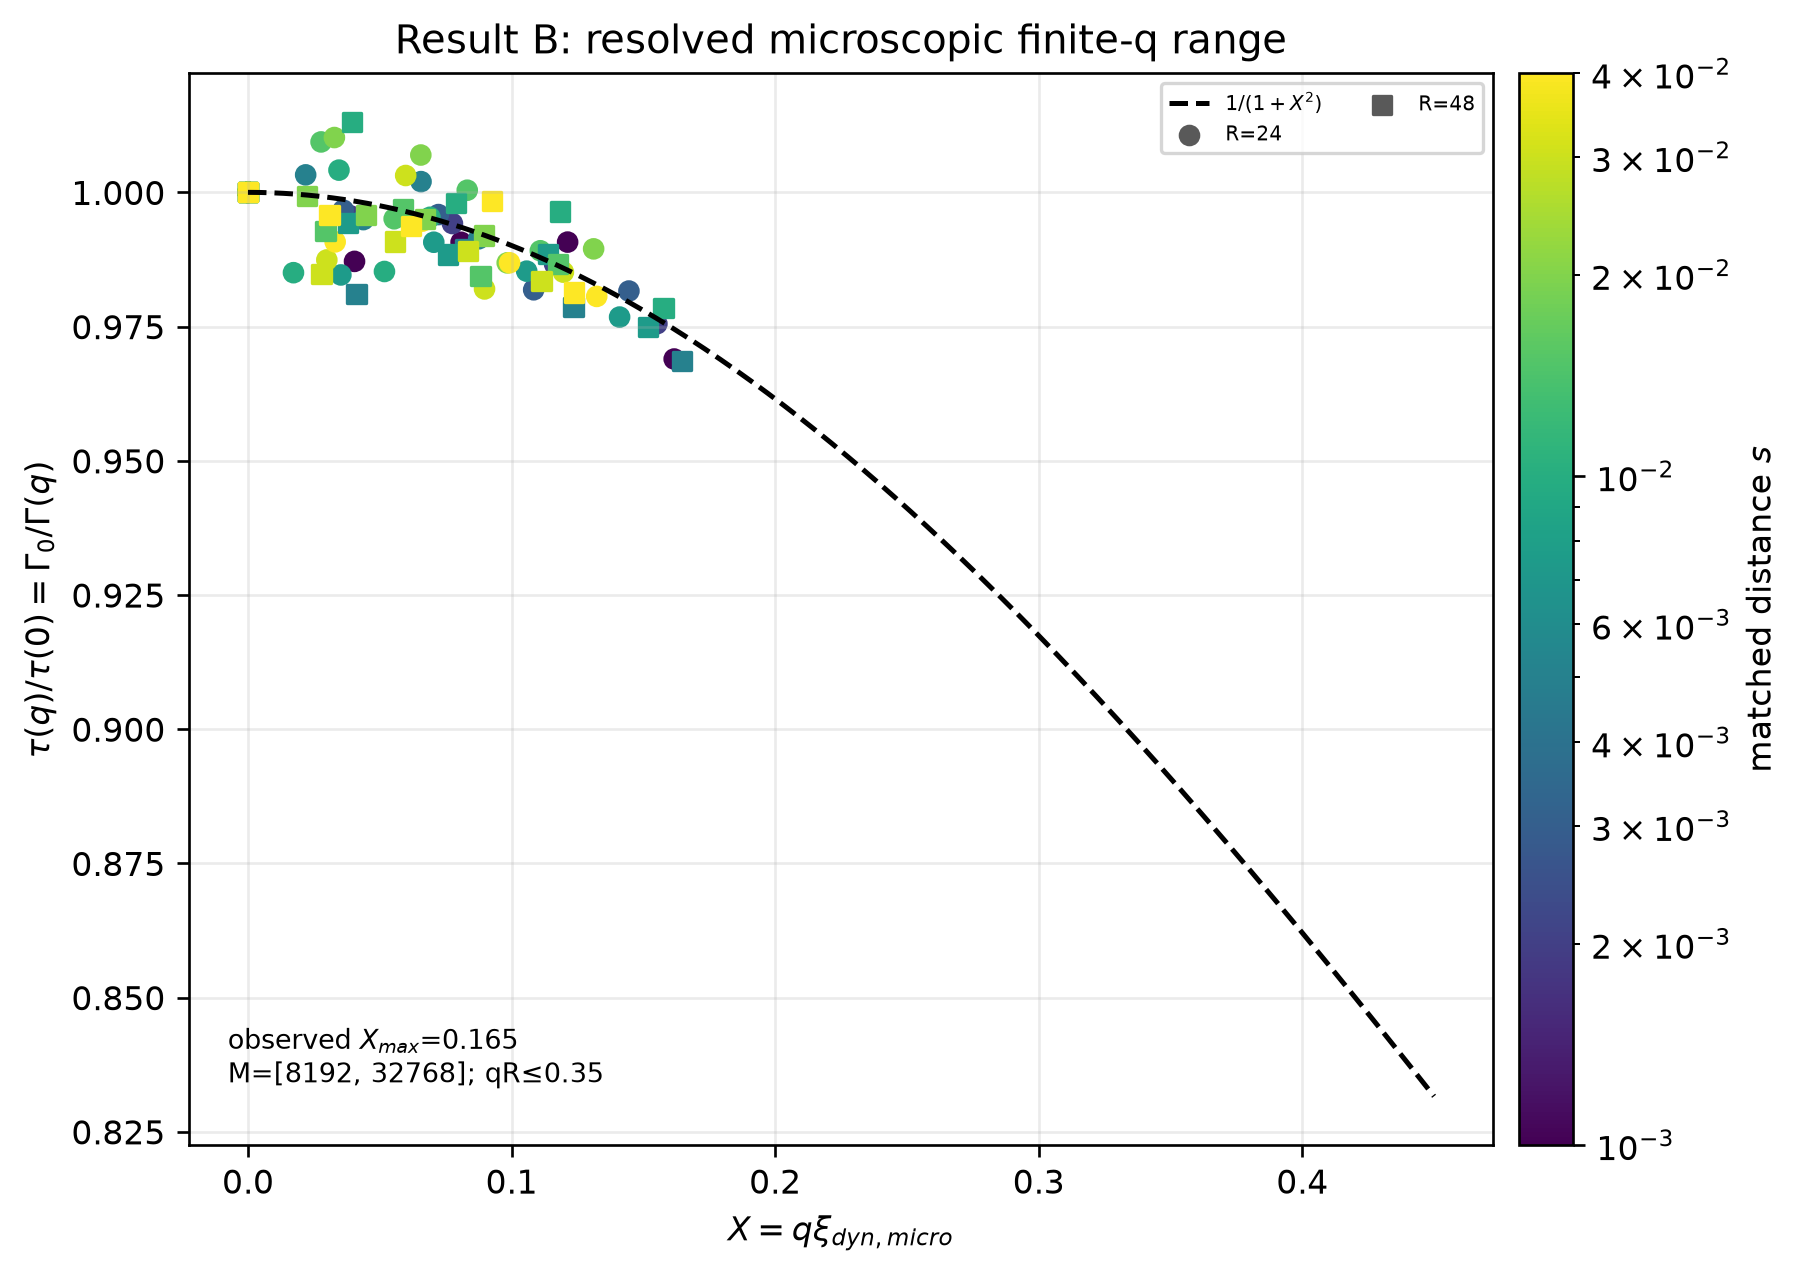
\includegraphics[width=0.91\linewidth]{figures/result1_finiteq.png}
\end{center}

円は$R=24$、四角は$R=48$、破線は長波長参照形$1/(1+X^2)$である。
解析窓は$qR\le0.35$、到達した最大値は$X_{\max}=0.165$である。
$q$が小さいほど広域な避難意思の偏り、$q$が大きいほど細かな局所的偏りを表す。
$\lambda(q)<0$なら同期更新ごとに\textbf{時間的に符号反転}するのであり、
空間的な逆向き伝播を意味しない。

\Caution{
  Result 1が直接示す中心的結果は、有限距離の微視的モデルにおける
  \textbf{規格化有限波数応答とkernel形状の整合}である。
  現在の微視的small-$q$データだけから、普遍的な$q^2$ dispersionを完全に実証したとは言わない。
  また、微視的横軸$s$を使う解析はoperational pseudospinodal近傍のeffective/matched解析であり、
  真の有限$R$ spinodal指数の証明ではない。
}

\section{正負一対の微小摂動と対称差分応答}\label{sec:symmetric}
\PosterMap{「数値検証｜有限距離の微視的モデル」の正負一対の微小摂動に対応。}

一様背景のまわりに
\begin{equation}
 u_i^{(\pm)}(0)=u^*\pm\epsilon\cos(qx_i)
 \label{eq:paired-initial}
\end{equation}
を与える。観測量$O(\epsilon)$をTaylor展開すると
\begin{align}
 O(+\epsilon)&=O(0)+O'(0)\epsilon+\frac12O''(0)\epsilon^2
 +\frac16O'''(0)\epsilon^3+\cdots,\\
 O(-\epsilon)&=O(0)-O'(0)\epsilon+\frac12O''(0)\epsilon^2
 -\frac16O'''(0)\epsilon^3+\cdots.
\end{align}
半差を取れば
\begin{equation}
 \boxed{O_{\mathrm{sym}}(\epsilon)
 \equiv\frac{O(+\epsilon)-O(-\epsilon)}2
 =O'(0)\epsilon+O(\epsilon^3)}.
 \label{eq:symmetric-difference}
\end{equation}
背景$O(0)$と偶数次非線形が消える。微視的計算で実際に使うprofile推定量は
\begin{equation}
 \widehat{\delta u}_i^{\mathrm{sym}}(t)
 =\frac{\bar S_i^{(+)}(t)-\bar S_i^{(-)}(t)}2,
 \qquad
 \bar S_i^{(\pm)}=\frac1M\sum_{\alpha=1}^{M}S_{i,\alpha}^{(\pm)}.
 \label{eq:numerical-symmetric-response}
\end{equation}

正負ペアには同じquenched閾値$\phi_i$と対応する乱数を使う。
\texttt{direct\_J}では各時刻・各bondの同じannealed $J_{ij}(t)$ realizationを
plus/minusで明示的に共有する。\texttt{aggregated\_exact}では$J_{ij}$を個別生成せず、
近傍和とplus/minus状態のoverlapから相関係数$\rho$を求め、同一$J$を共有した二つの局所場の
条件付きjoint Gaussian統計を二つの標準Gaussian乱数から厳密に再構成する。
これは共通乱数による分散低減に効く。ただし中心は、対称差分によって
\textbf{背景と偶数次成分を除き、線形応答を抽出すること}である。

\section{長波長展開と\texorpdfstring{$\kappa_R$}{kappa-R}}\label{sec:kappa}
\PosterMap{「理論｜長波長展開」と「係数の相互作用範囲依存性」に対応。}

条件$|q|Ra\ll1$で$\cos(qra)$を展開する。
\begin{align}
 K_R(q)
 &=\frac1R\sum_{r=1}^{R}
 \left[1-\frac{(qra)^2}{2}+O(q^4r^4a^4)\right]\\
 &=1-\frac{q^2a^2}{2R}\sum_{r=1}^{R}r^2+O(q^4).
\end{align}
\begin{equation}
 \sum_{r=1}^{R}r^2=\frac{R(R+1)(2R+1)}6
\end{equation}
を代入すると
\begin{align}
 \boxed{K_R(q)=1-\kappa_Rq^2+O(q^4)},\label{eq:kernel-longwave}\\
 \boxed{\kappa_R=\frac{a^2(R+1)(2R+1)}{12}}.
 \label{eq:kappa-R}
\end{align}

$\kappa_R$はfitパラメータではなく、top-hat kernelから解析的に決まる係数である。
大きな$R$では$\kappa_R\sim a^2R^2/6$となる。

\section{\texorpdfstring{$\Gamma(q)=\Gamma_0+\kappa_Rq^2$}{Gamma(q) = Gamma-zero + kappa-R q-squared}}\label{sec:dispersion}
\PosterMap{「理論｜長波長展開」から特徴的空間長へ進む中間式。}

離散時間のモード倍率を連続的な減衰率へ変換するため
\begin{equation}
 \Gamma(q)\equiv-\ln|\lambda(q)|,
 \qquad \Gamma_0\equiv-\ln\Lambda^*
 \label{eq:gamma-definition}
\end{equation}
と定義する。$q=0$近傍で$K_R(q)>0$なら
\begin{align}
 \Gamma(q)
 &=-\ln\Lambda^*-\ln K_R(q)\\
 &=\Gamma_0-\ln\left[1-\kappa_Rq^2+O(q^4)\right]\\
 &=\boxed{\Gamma_0+\kappa_Rq^2+O(q^4)}.
 \label{eq:gamma-dispersion}
\end{align}

$\lambda(q)<0$のモードは時刻ごとに符号反転するため、絶対値を取った
$\Gamma=-\ln|\lambda|$が振幅包絡の減衰率となる。

\Caution{
  式\eqref{eq:gamma-dispersion}は局所平均意思のGaussian closureと
  $|q|Ra\ll1$から得る長波長予測である。
  Result 1の微視的有限波数スペクトルに対する普遍的実証とは区別する。
}

\section{特徴的空間長\texorpdfstring{$\xi$}{xi}}\label{sec:xi}
\PosterMap{「理論｜特徴的な空間長」とResult 3のbulk指数減衰に対応。}

\subsection{有限\texorpdfstring{$R$}{R}格子上のcharacteristic equation}

まず連続体近似をせず、本研究のtop-hat kernelから直接始める。
bulkで定常な線形応答は式\eqref{eq:spatial-linear}の左右の時刻を等しくして
\begin{equation}
 \delta u_i
 =\frac{\Lambda^*}{2R}\sum_{r=1}^{R}
 \left(\delta u_{i+r}+\delta u_{i-r}\right)
 \label{eq:lattice-stationary}
\end{equation}
を満たす。半無限bulkの減衰mode
\begin{equation}
 \delta u_i=A\exp(-x_i/\xi_{\mathrm{lat}}),
 \qquad x_i=ia
\end{equation}
を代入すると
\begin{align}
 \delta u_{i+r}
 &=\delta u_i\exp(-ra/\xi_{\mathrm{lat}}),\\
 \delta u_{i-r}
 &=\delta u_i\exp(+ra/\xi_{\mathrm{lat}}).
\end{align}
$\delta u_i\neq0$で割り、$\cosh y=(\e^y+\e^{-y})/2$を使えば
\begin{equation}
 \boxed{
  1=\Lambda^*\frac1R\sum_{r=1}^{R}
  \cosh\!\left(\frac{ra}{\xi_{\mathrm{lat}}}\right)}
 \label{eq:finite-R-characteristic}
\end{equation}
を得る。これは\textbf{有限$R$格子上の線形bulk characteristic equation}であり、
本研究のfinite-$R$ kernelから直接導いた式である。線形化・並進対称bulk・単一指数modeの
範囲では$R$を展開していない。一方、境界層や有限右端の反射はこの式には含まない。

\subsection{長波長有限\texorpdfstring{$R$}{R}近似}

$\xi_{\mathrm{lat}}\gg Ra$なら
\begin{equation}
 \cosh\!\left(\frac{ra}{\xi_{\mathrm{lat}}}\right)
 =1+\frac{r^2a^2}{2\xi_{\mathrm{lat}}^2}
 +O\!\left[\left(\frac{Ra}{\xi_{\mathrm{lat}}}\right)^4\right].
\end{equation}
式\eqref{eq:kappa-R}を用いると
\begin{equation}
 1=\Lambda^*\left[1+\frac{\kappa_R}{\xi_{\mathrm{lat}}^2}
 +O\!\left\{(Ra/\xi_{\mathrm{lat}})^4\right\}\right]
\end{equation}
であり、主要項から
\begin{align}
 \boxed{\xi_{\mathrm{lat}}^2
 \simeq\frac{\Lambda^*\kappa_R}{1-\Lambda^*}}
 &=\boxed{\frac{\kappa_R}{\exp(\Gamma_0)-1}},
 \qquad \Lambda^*=\e^{-\Gamma_0}.
 \label{eq:xi-lattice-longwave}
\end{align}

\subsection{spinodal近傍の漸近長}

$\Gamma_0\ll1$では
\begin{equation}
 \e^{\Gamma_0}-1=\Gamma_0+\frac12\Gamma_0^2+\cdots
\end{equation}
なので、連続体・長波長の漸近予測を
\begin{equation}
 \boxed{\xi_{\Gamma}\equiv\sqrt{\frac{\kappa_R}{\Gamma_0}}},
 \qquad \xi_{\mathrm{lat}}\sim\xi_{\Gamma}
 \label{eq:xi-Gamma}
\end{equation}
と定義する。この段階で初めて
\begin{equation}
 \left(\Gamma_0-\kappa_R\partial_x^2\right)\delta u(x)=0
 \label{eq:continuum-boundary}
\end{equation}
という連続体式が得られる。固定境界の実profileから独立にfitする数値長は
$\xi_{\bnd}$、境界条件別のbulk fit長は$\xi_{\bulk}$と書き、
$\xi_{\mathrm{lat}}$や$\xi_{\Gamma}$と区別する。

\Meaning
{格子式\eqref{eq:finite-R-characteristic}の正根が減衰長を決め、その長波長極限が$\xi_{\Gamma}$である。}
{復元力が弱いほど、局所摂動の影響は長い距離まで残る。}
{一端の避難意思や局所情報が、集団内部へどこまで浸透して減衰するかを表す。}

\section{\texorpdfstring{$\xi\propto\delta^{-1/4}$}{xi proportional to delta to the minus one-quarter}}\label{sec:xi-scaling}
\PosterMap{「理論｜特徴的な空間長」のspinodal scalingを補足。}

固定$R$では$\kappa_R$は$\delta_{\Gauss}$に依存しない。
式\eqref{eq:gamma-sqrt}を漸近長\eqref{eq:xi-Gamma}へ代入すると
\begin{equation}
 \boxed{\xi_{\Gamma}\propto
 \left(\delta_{\Gauss}^{1/2}\right)^{-1/2}
 =\delta_{\Gauss}^{-1/4}}.
 \label{eq:xi-quarter}
\end{equation}

指数$-1/4$は、spinodalの時間方向の$1/2$乗と、空間勾配が$q^2$で始まることの
組合せから生じる。境界profileからfitした数値結果では、固定窓
$\delta_{\Gauss}\le3\times10^{-4}$で$R=6,12,24,48,96$の有効指数が
およそ$-0.254$から$-0.257$である。これは有限距離での近接を示す数値結果であり、
無限精度の指数決定ではない。

\section{\texorpdfstring{$\tau_0\propto\xi^2$}{tau-zero proportional to xi-squared}と\texorpdfstring{$z=2$}{z = 2}}\label{sec:z2}
\PosterMap{「理論」の最下段と「結果2｜臨界近傍の時間・空間スケーリング」に対応。}

理論上は定義\eqref{eq:xi-Gamma}を整理すると
\begin{equation}
 \boxed{\tau_0\equiv\Gamma_0^{-1}
 =\frac{\xi_{\Gamma}^2}{\kappa_R}}.
 \label{eq:tau-xi}
\end{equation}
固定$R$では$\kappa_R$が定数なので
\begin{equation}
\tau_0\propto\xi_{\Gamma}^{z},\qquad \boxed{z=2}.
 \label{eq:z-two}
\end{equation}

一方、固定境界profileから独立fitした$\xi_{\bnd}$には定義上の等号はない。
数値検証は
\begin{equation}
 \boxed{\tau_{0,\mathrm{num}}
 \simeq\frac{\xi_{\bnd}^2}{\kappa_R}}
 \label{eq:tau-xi-numeric-test}
\end{equation}
が成り立つかを別protocol間で調べる\textbf{consistency test}である。

この$z=2$は、非保存的な局所緩和と解析的な$q^2$勾配項から得るGaussian長波長予測である。
動的臨界現象の一般的背景はHohenberg--Halperinの分類\cite{hohenberg1977}を参照する。

\Caution{
  本研究がModel A universality classに属することを証明したわけではない。
  ここで確認しているのは、指定した決定論的Gaussian closureの長波長線形応答における
  $z=2$予測と、その数値的整合である。
}

\section{\texorpdfstring{$R$}{R}をまたぐ規格化とResult 2}\label{sec:result2}
\PosterMap{「結果2｜臨界近傍の時間・空間スケーリング」の主図と注記に対応。}

$R$が変わると式\eqref{eq:kappa-R}も変わるため、生の$\xi_{\bnd}$を同じ横軸に重ねるだけでは
kernel由来のoffsetが残る。そこで解析的規格化
\begin{equation}
 \widetilde\xi\equiv\frac{\xi_{\bnd}}{\sqrt{\kappa_R}}
 \label{eq:xi-scaled}
\end{equation}
を用いる。有限$R$数値データが長波長予測に従えば
\begin{equation}
 \boxed{\tau_{0,\mathrm{num}}\simeq\widetilde\xi^{\,2}}
 \label{eq:normalized-z}
\end{equation}
となる。$\sqrt{\kappa_R}$はfitで合わせた尺度ではなく、有限距離kernelから解析的に決まる。

\subsection{\texorpdfstring{$R$}{R} sweepで固定する量}

Result 2では$B=2$、$\sigma_J=1$、$\sigma_\phi=0.06$、$\bar\phi=0$、
$a=1$、stay-to-evacuate枝、$\epsilon_{\mathrm{fraction}}=0.05$を固定した。
$N$は$R=6,12,24,48,96$に対し$512,1024,2048,4096,8192$とした。
ただし
\begin{align}
 \sigma_{\mathrm{eff}}^2(R)
 &=\frac{\sigma_J^2}{2R}+\sigma_\phi^2,\\
 B&=\frac{2\mu}{\sqrt{2\pi}\sigma_{\mathrm{eff}}}
 \quad\Longrightarrow\quad
 \boxed{\mu(R)=\frac{B\sqrt{2\pi}}2\sigma_{\mathrm{eff}}(R)}
 \label{eq:mu-fixed-B}
\end{align}
なので、$\mu$は固定していない。

\begin{center}\small
\begin{tabular}{rrrr}
\toprule
$R$ & $N$ & $\sigma_{\mathrm{eff}}(R)$ & $\mu(R)$ \\
\midrule
6  & 512  & 0.294845 & 0.739066 \\
12 & 1024 & 0.212760 & 0.533309 \\
24 & 2048 & 0.156312 & 0.391815 \\
48 & 4096 & 0.118392 & 0.296765 \\
96 & 8192 & 0.093853 & 0.235254 \\
\bottomrule
\end{tabular}
\end{center}

無次元距離を
\begin{equation}
 \widetilde\delta\equiv\frac{\delta_{\Gauss}}{\sigma_{\mathrm{eff}}(R)}
 \label{eq:reduced-delta}
\end{equation}
とすれば、同じabsolute $\delta_{\Gauss}$でも完全に同じ無次元距離ではない。
例えば$\delta_{\Gauss}=10^{-5}$では$\widetilde\delta=3.39\times10^{-5}$から
$1.07\times10^{-4}$まで変わる。これは有限窓での$R$依存driftを読む際の注意である。

% POSTER DEFINITION: Result 2は同一closure内の別protocol・別observableによる整合性検証。
\subsection{時間量と空間量を別々に測る}

時間量は周期境界の$q=0$緩和を直接計算し、原点通過fit
\begin{equation}
 A_0(t+1)=\lambda_{\mathrm{fit}}(0)A_0(t)
 \label{eq:q0-direct-fit}
\end{equation}
から
\begin{equation}
 \Gamma_{0,\mathrm{num}}=-\ln|\lambda_{\mathrm{fit}}(0)|,
 \qquad \tau_{0,\mathrm{num}}=1/\Gamma_{0,\mathrm{num}},
 \label{eq:tau-numeric}
\end{equation}
を測定した。空間量は固定境界profileのcosh fitから$\xi_{\bnd}$として\textbf{別に}測定した。
$\xi_{\bnd}$を$\sqrt{\kappa_R/\Gamma_0}$から計算してはいない。

\begin{center}
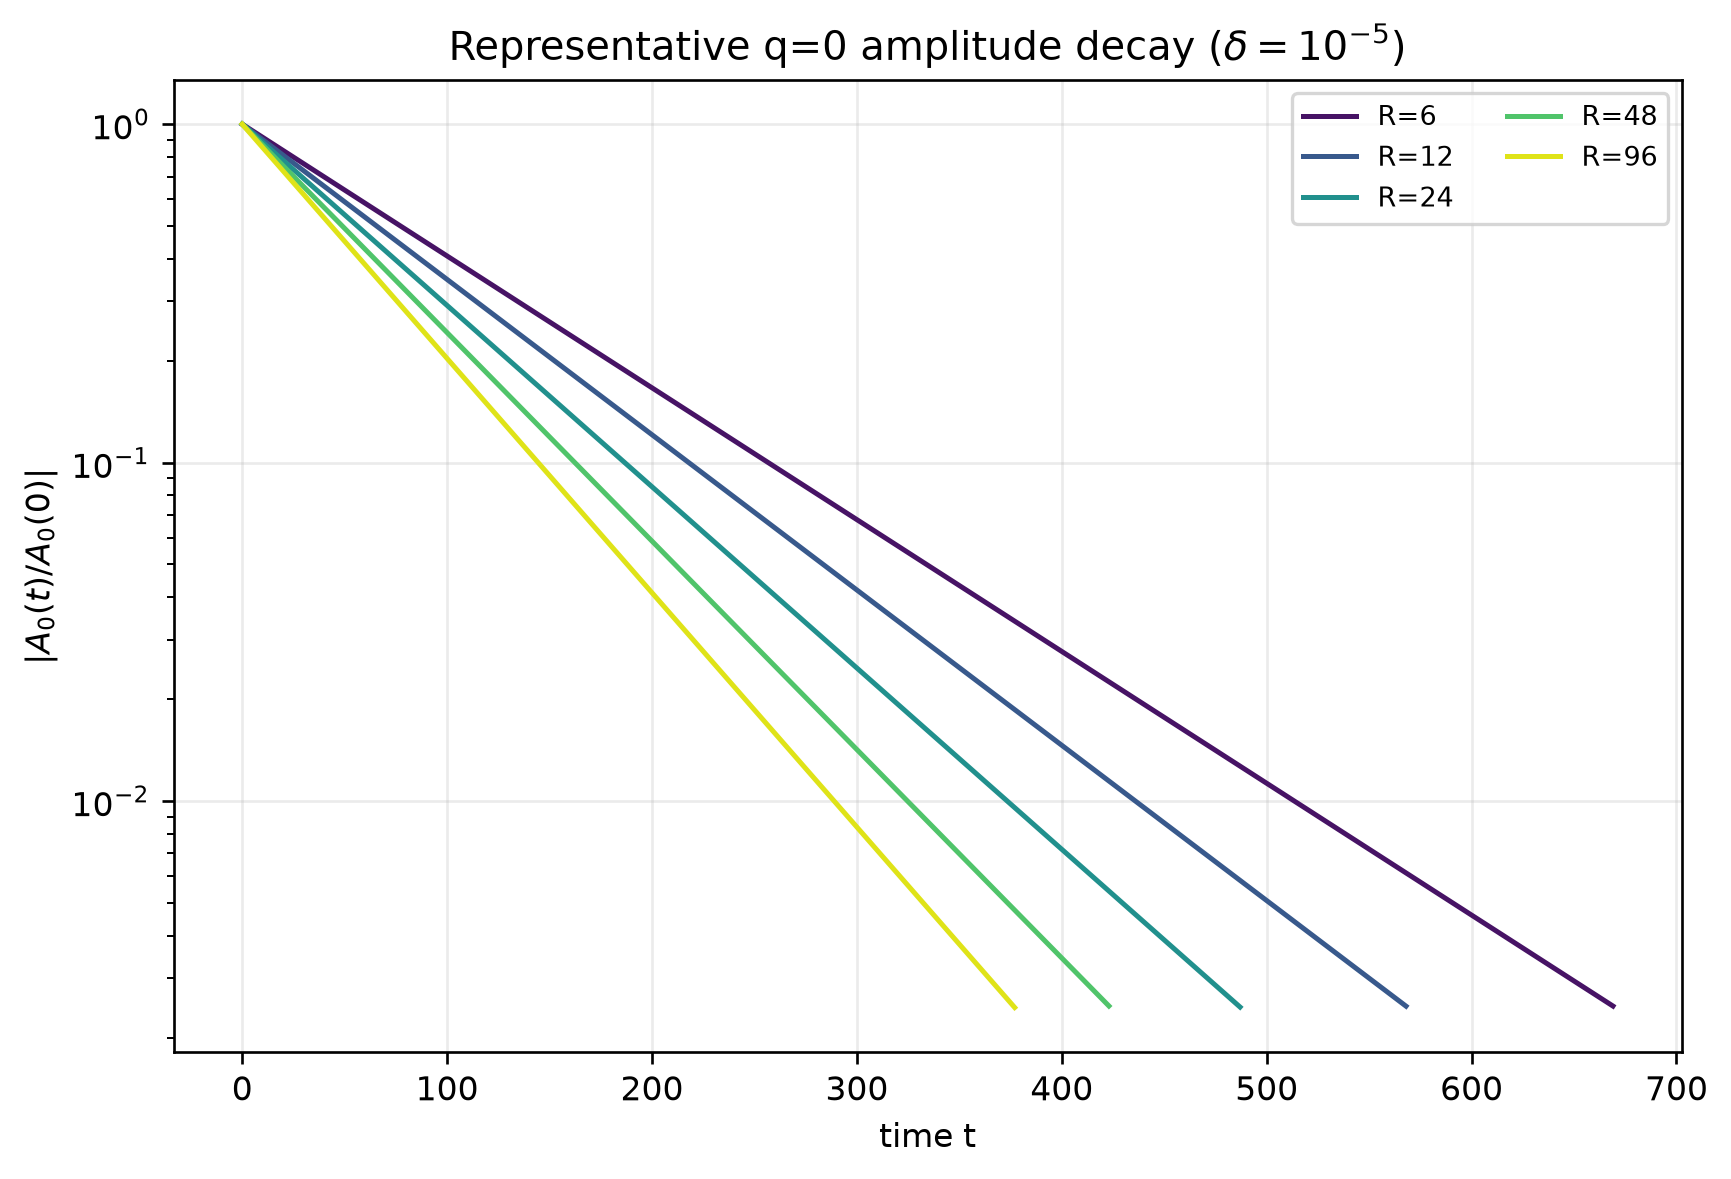
\includegraphics[width=0.84\linewidth]{figures/result2_q0_decay.png}
\end{center}

半対数上の直線性が直接測定の内容である。さらに全条件の
$\Gamma_{0,\mathrm{num}}$と写像微分の理論値を比較すると次図のようになる。

\begin{center}
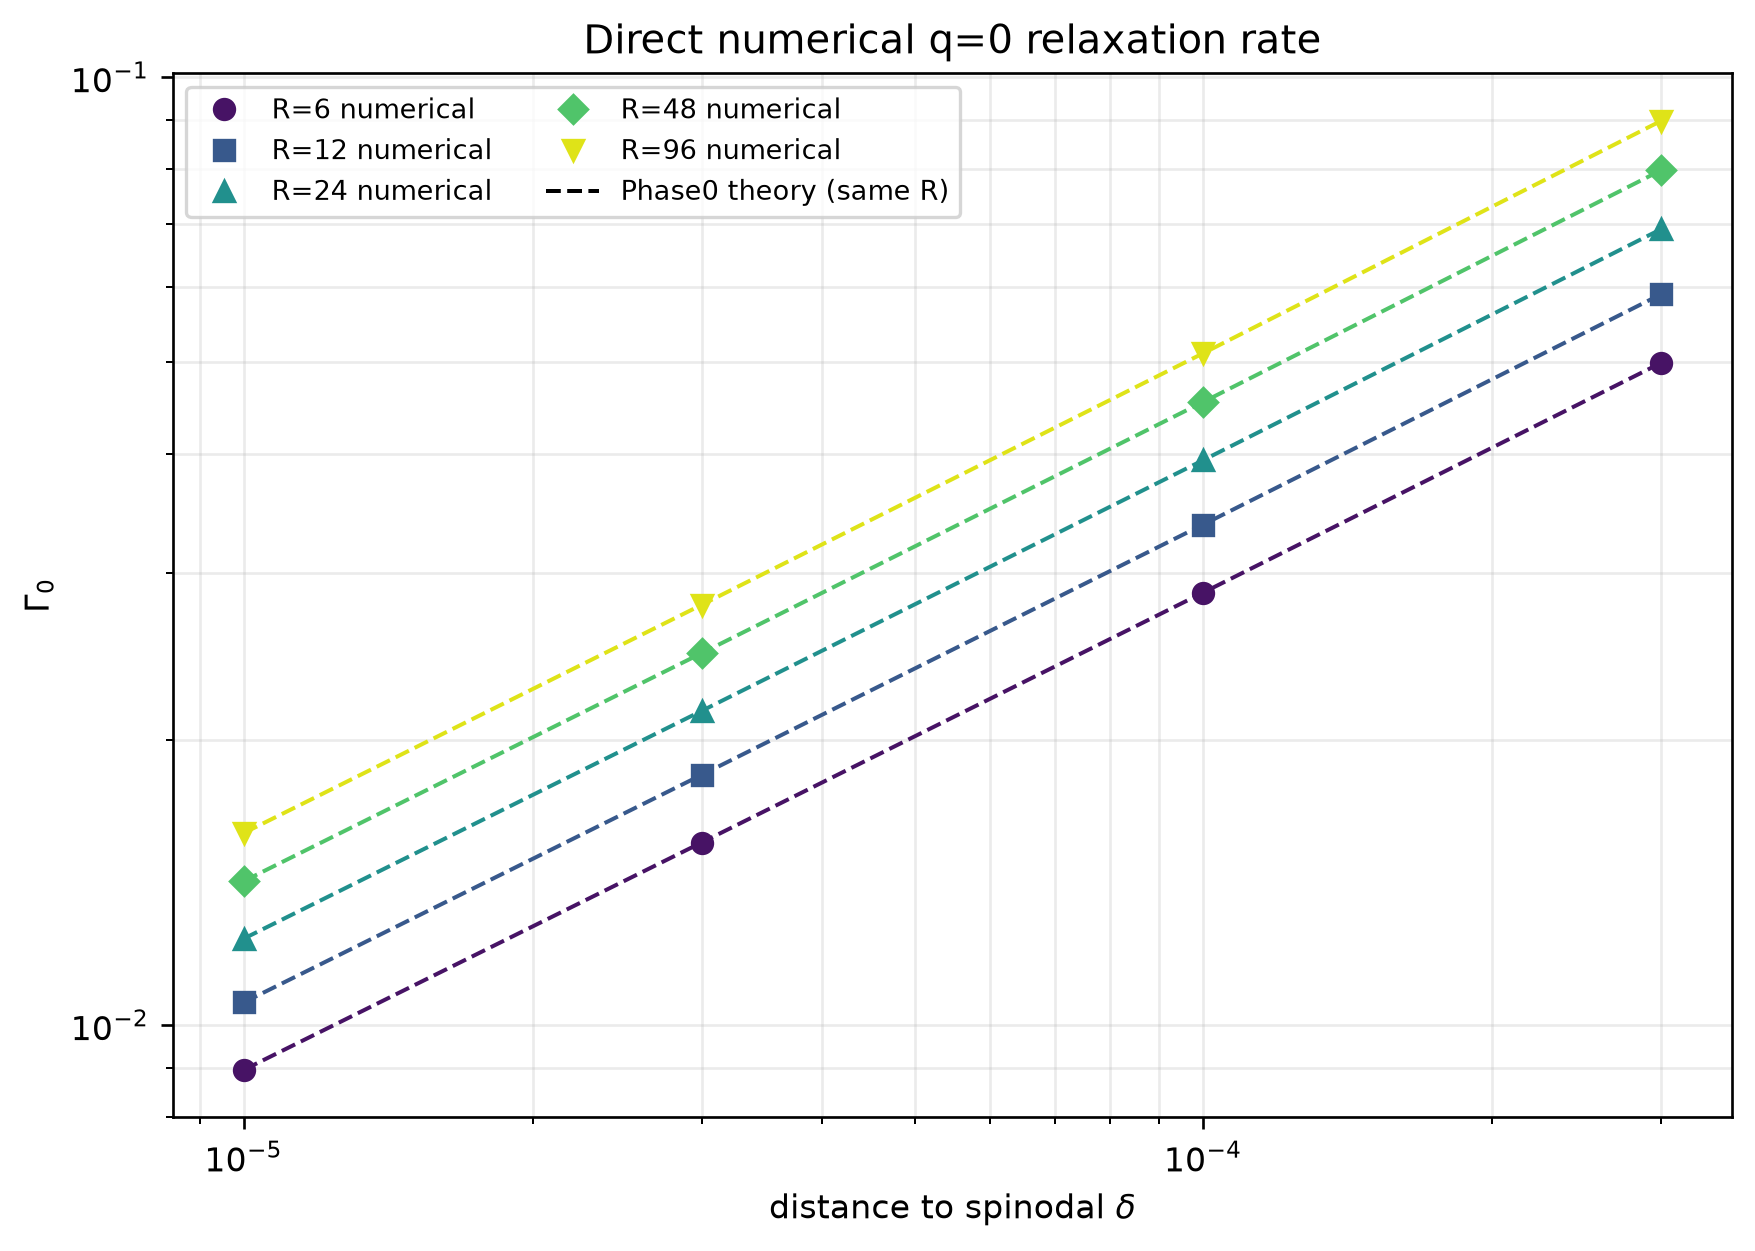
\includegraphics[width=0.82\linewidth]{figures/result2_q0_gamma.png}
\end{center}

\subsection{raw座標とkernel規格化座標}

\begin{center}
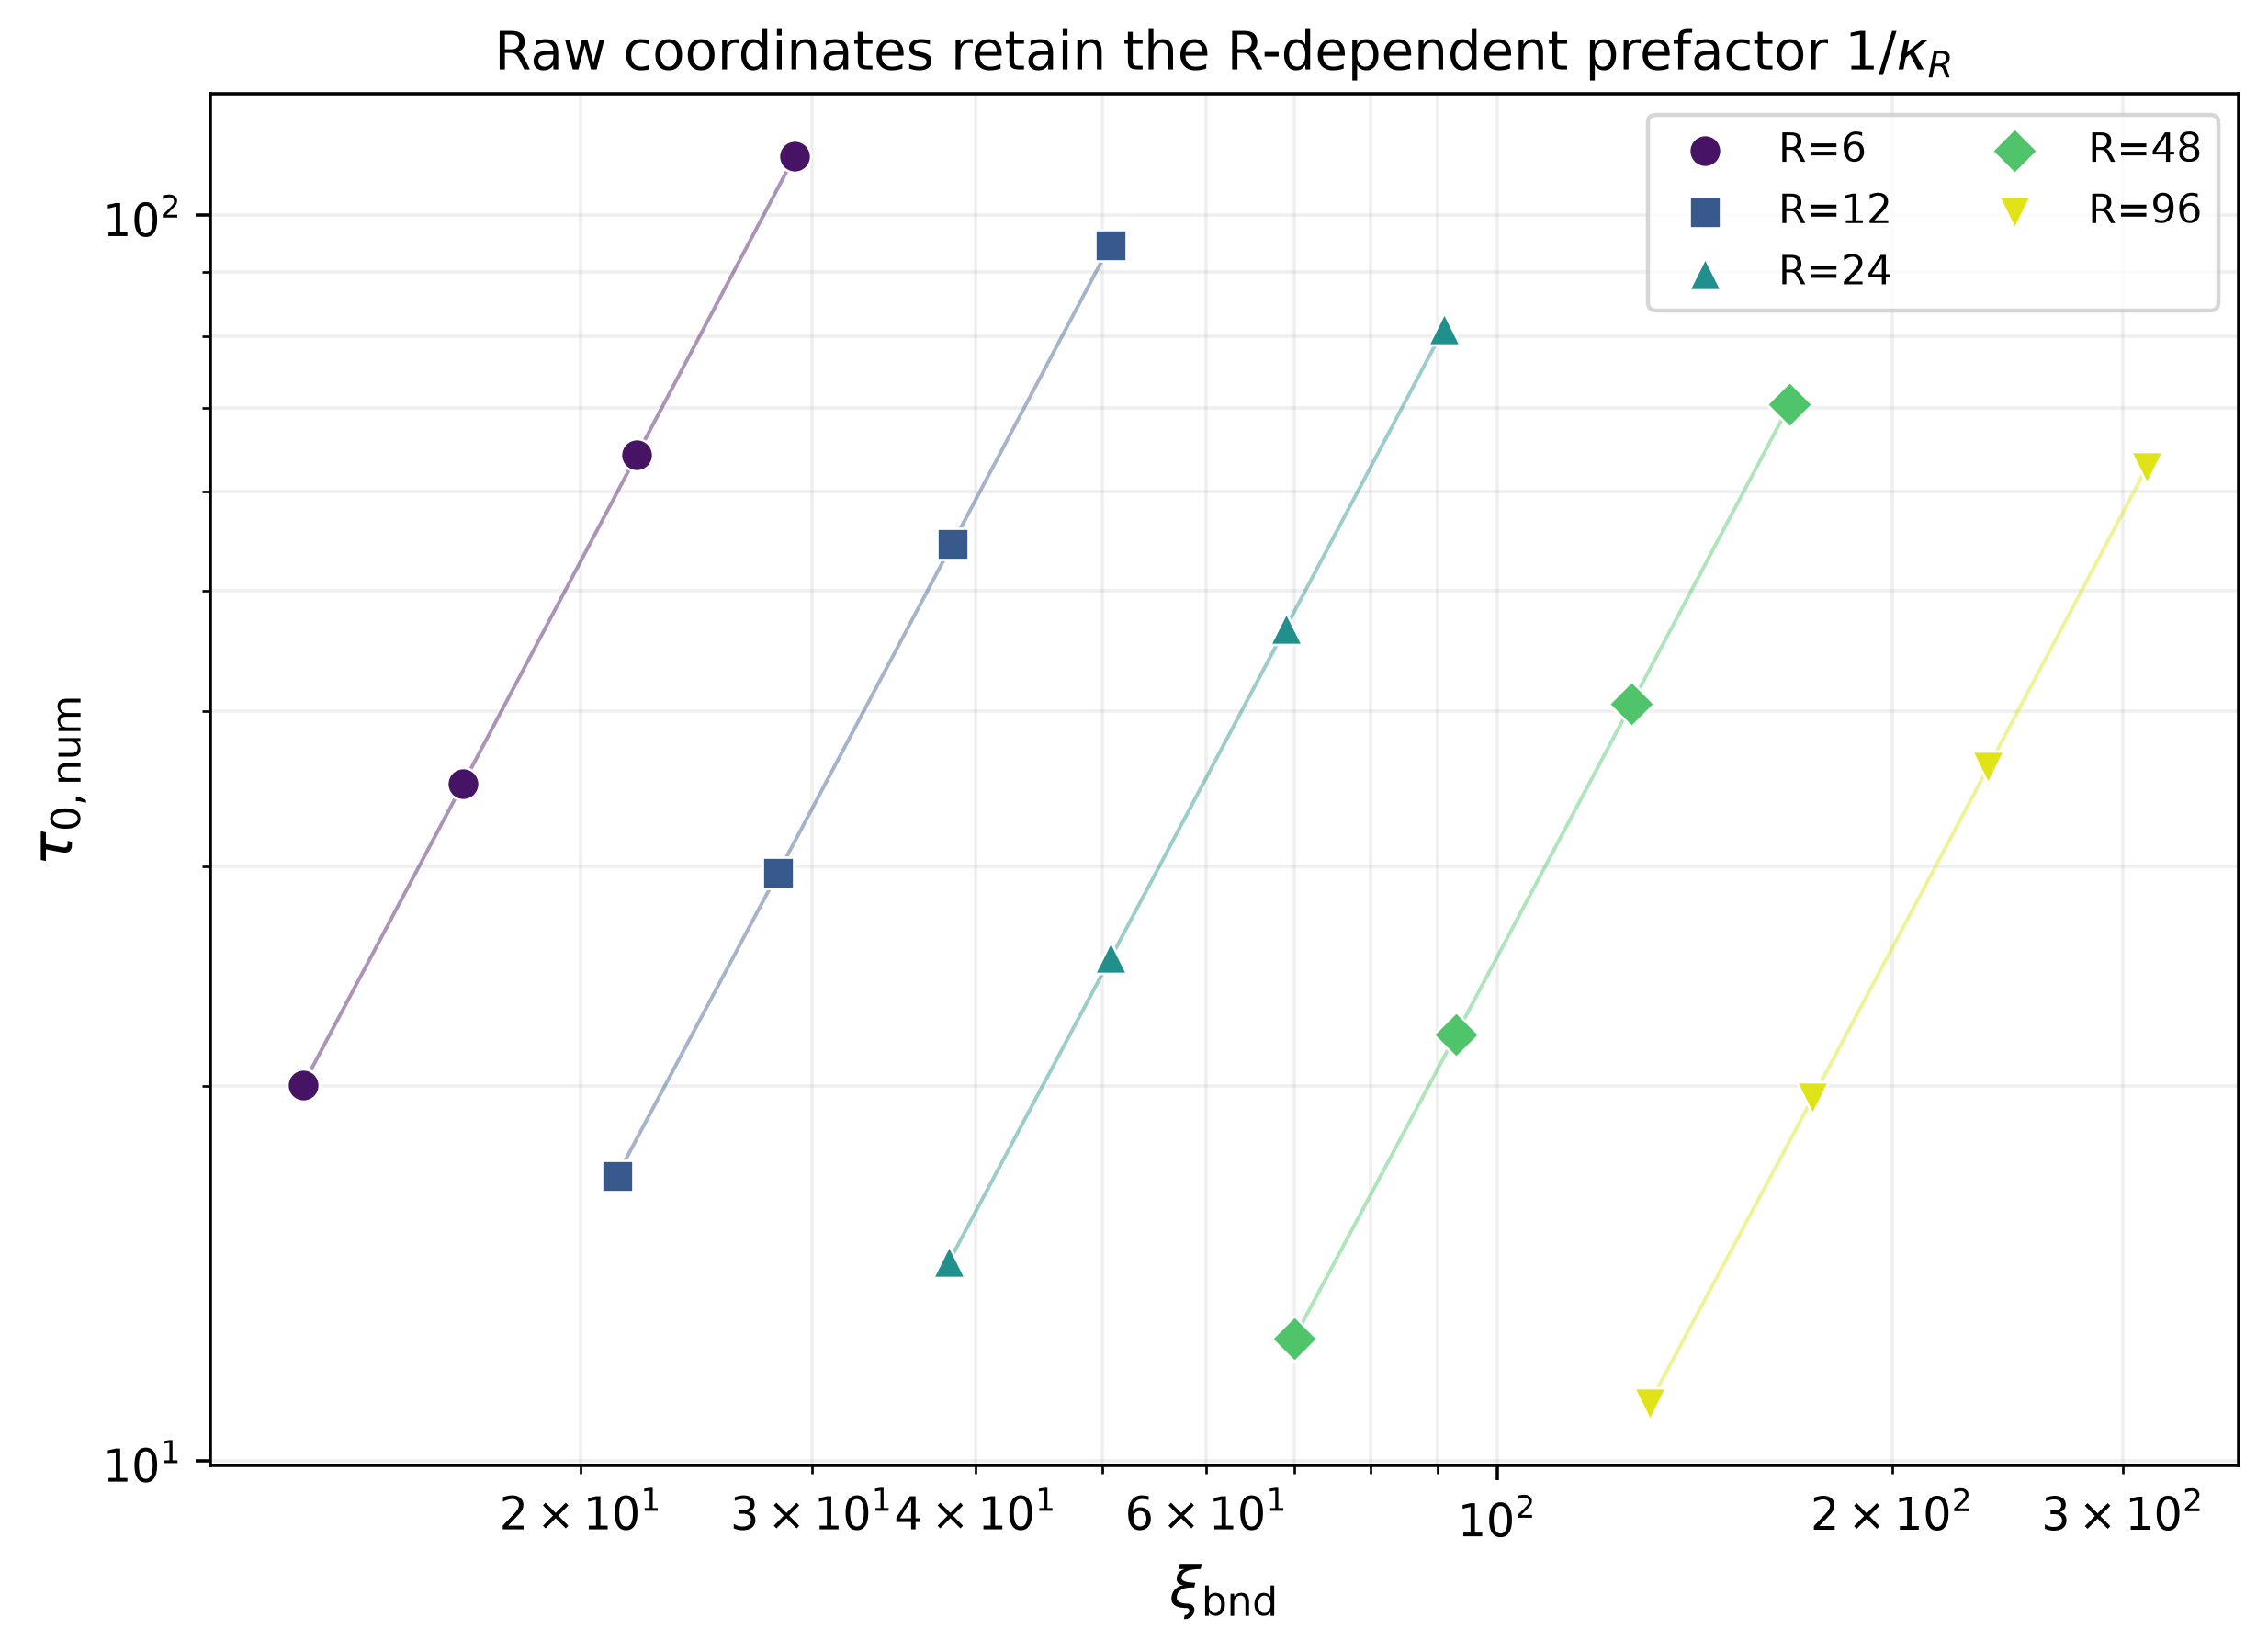
\includegraphics[width=0.91\linewidth]{figures/result2_raw.png}
\end{center}

raw座標では理論関係$\tau\sim\xi^2/\kappa_R$の$1/\kappa_R$が$R$ごとに異なるため、
系列間にoffsetが残る。

\begin{center}
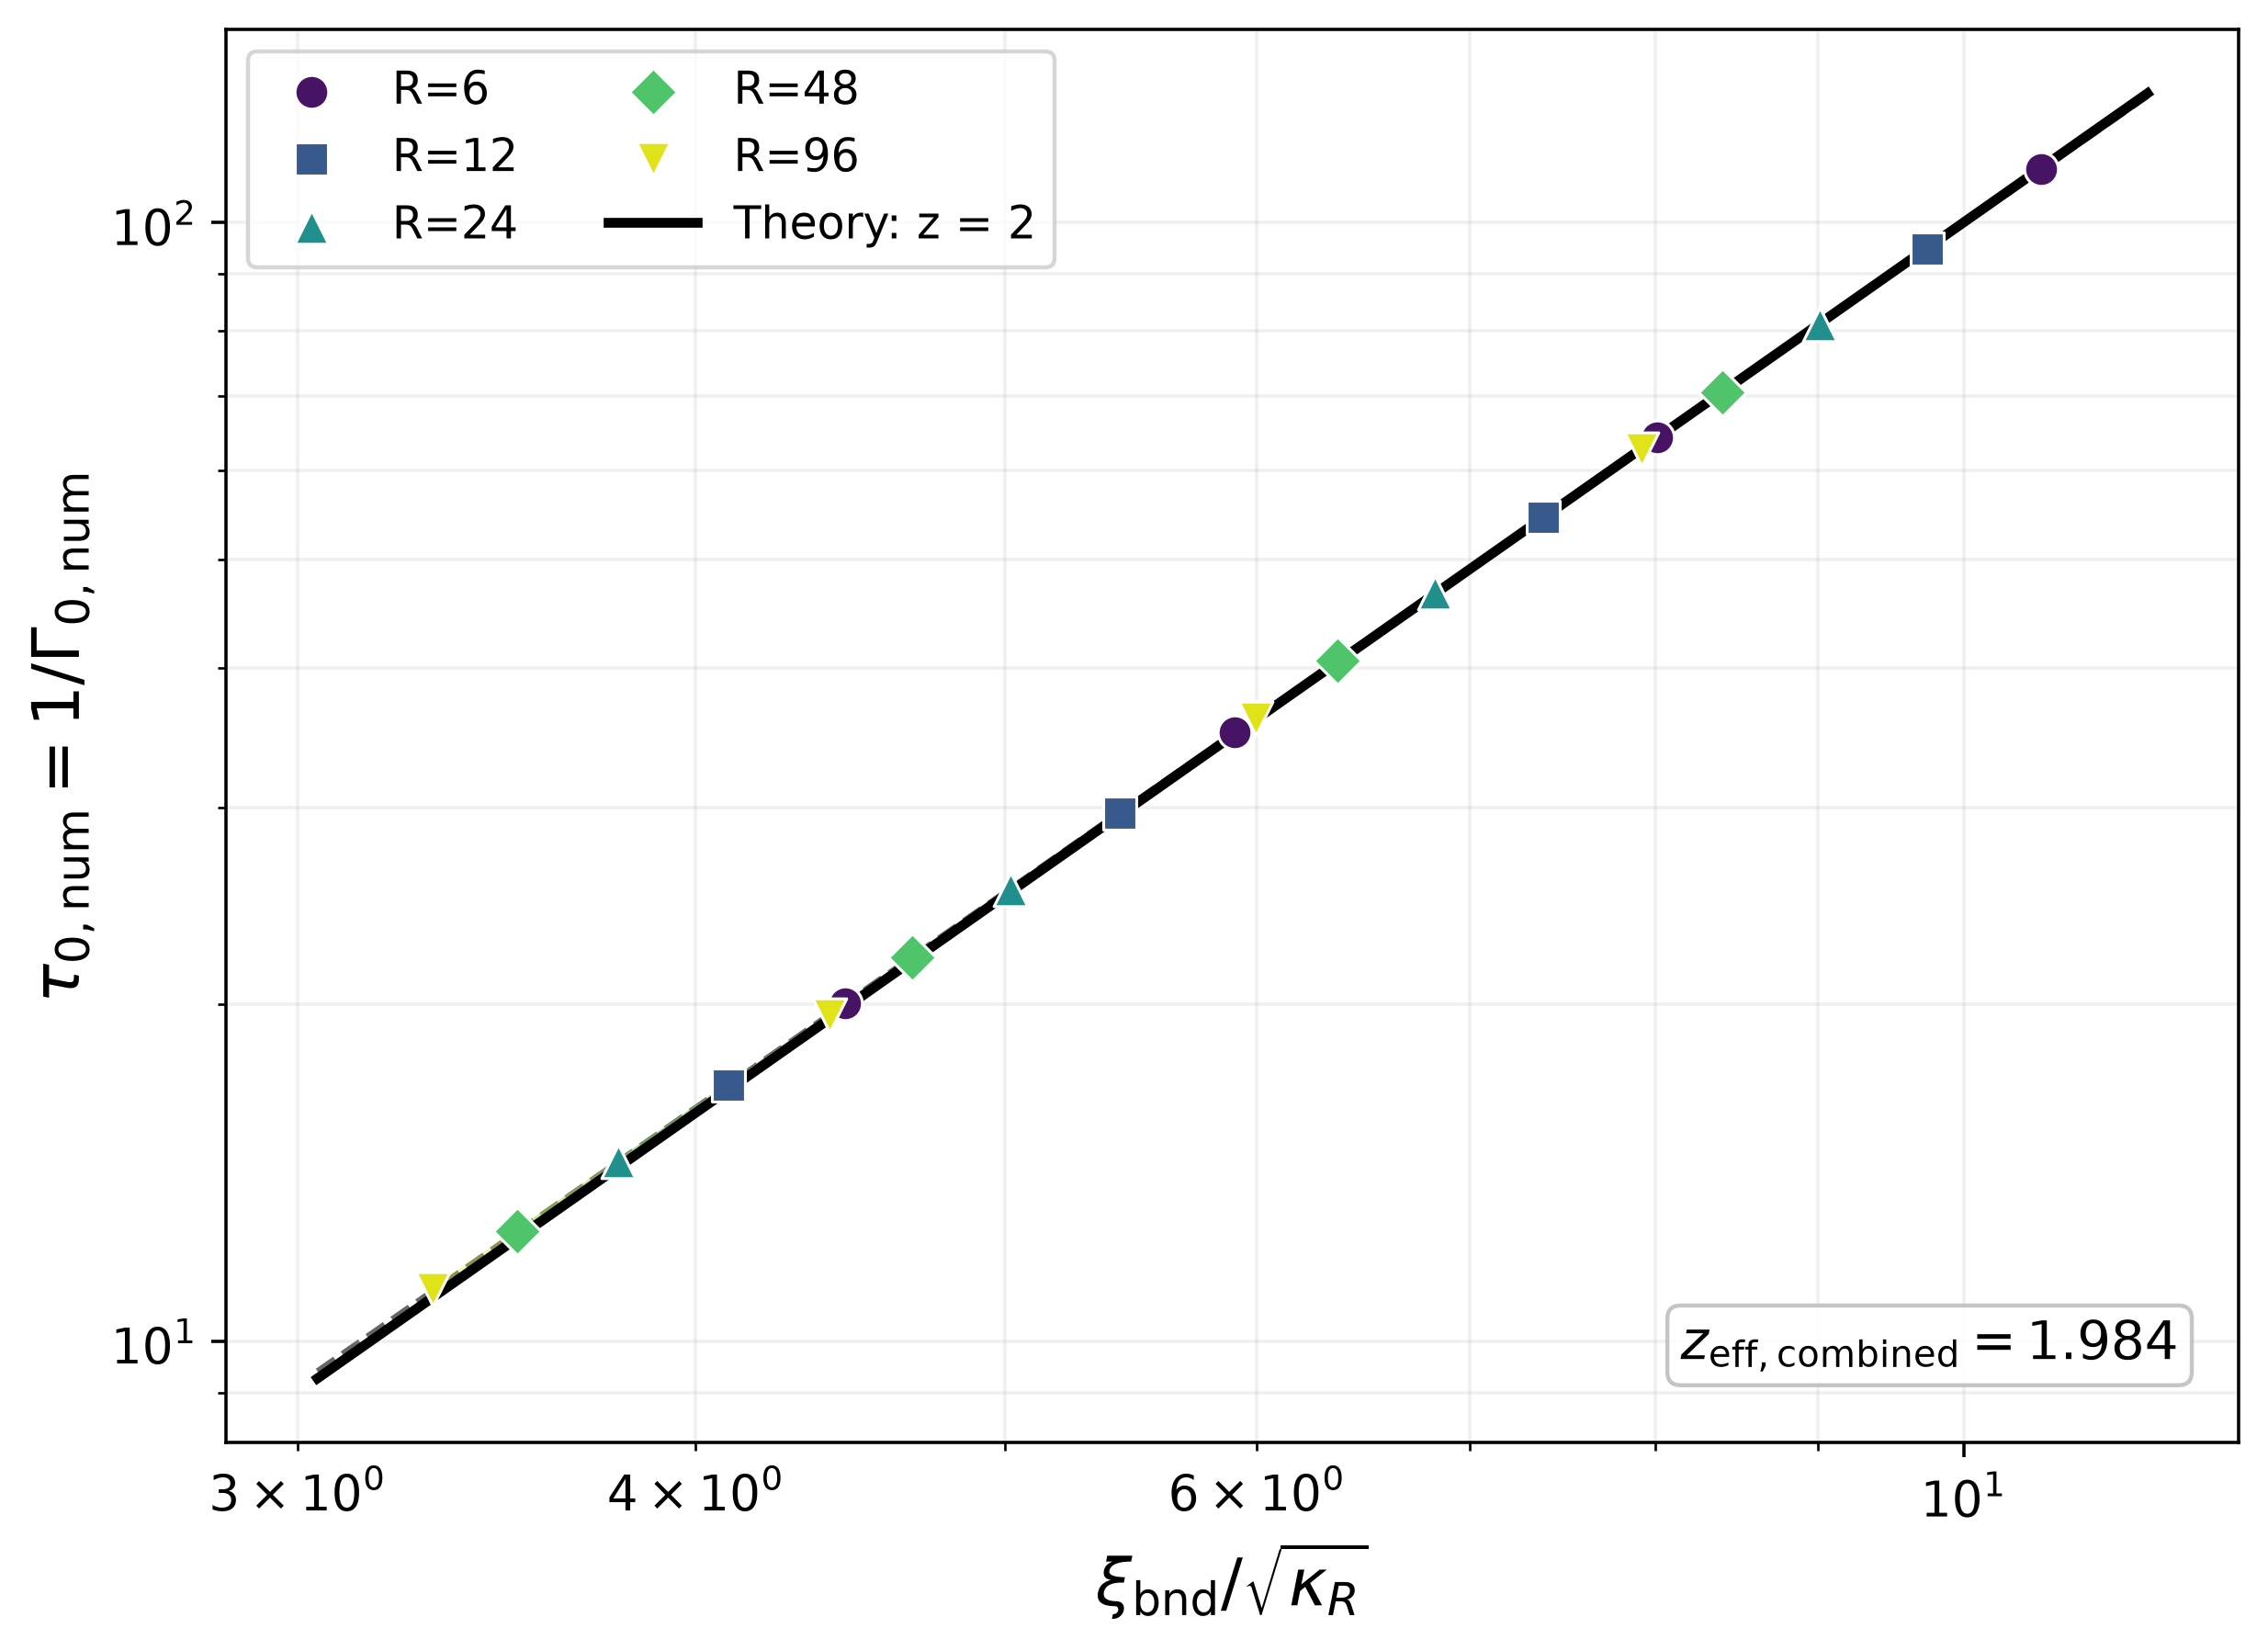
\includegraphics[width=0.91\linewidth]{figures/result2_normalized.png}
\end{center}

$\xi_{\bnd}/\sqrt{\kappa_R}$で既知のkernel依存を除くと共通曲線へ重なる。
全20点の有限窓fitは$z_{\mathrm{eff}}=1.9842$、
最近接10点では$1.9907$で、spinodalへ近い窓ほど漸近値2へ近づく。
また$\kappa_R\tau_{0,\mathrm{num}}/\xi_{\bnd}^2$の1からの最大偏差は約$1.68\%$である。
このような有限窓のdriftは広い意味でのcorrections to scalingとして整理できる
\cite{wegner1972}が、本非平衡離散写像の補正指数をWegnerの平衡理論と同一視はしない。

\clearpage
\subsection{finite-\texorpdfstring{$R$}{R}格子長との独立比較}

各点の$\Gamma_{0,\mathrm{num}}$から$\Lambda_{\mathrm{num}}=\e^{-\Gamma_{0,\mathrm{num}}}$を作り、
式\eqref{eq:finite-R-characteristic}を数値的に解いた。

\begin{center}
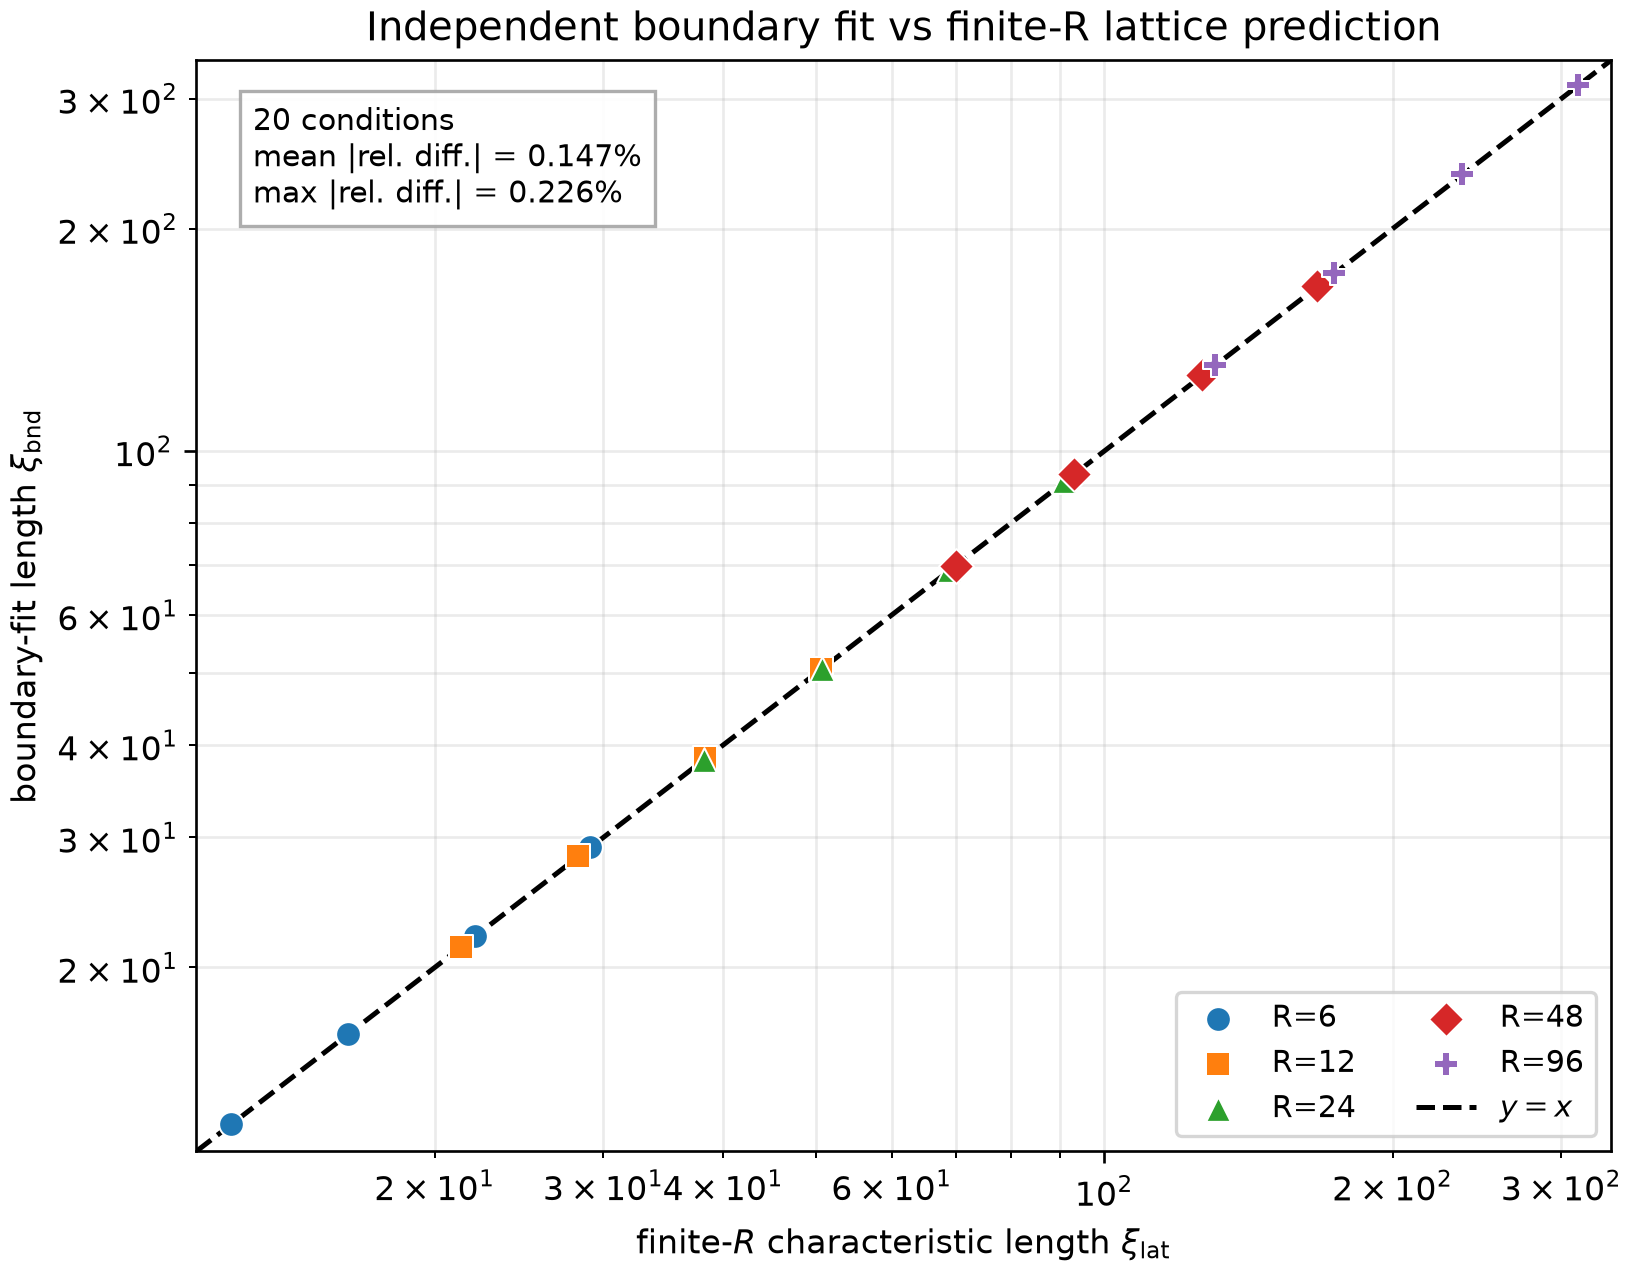
\includegraphics[width=0.74\linewidth]{figures/xi_lat_vs_xi_bnd.png}
\end{center}

finite-$R$格子のcharacteristic equationによる$\xi_{\mathrm{lat}}$は、
fixed-boundary profileから独立にfitした$\xi_{\bnd}$と全20条件でよく一致する。
$|\xi_{\bnd}/\xi_{\mathrm{lat}}-1|$の平均は$0.147\%$、最大は$0.226\%$
（$R=6$, $\delta_{\Gauss}=10^{-5}$）である。
再計算値は\texttt{data/xi\_lat\_vs\_xi\_bnd.csv}、生成手順は
\texttt{make\_support\_figures.py}に保存した。

\Caution{
  データは決定論的である。回帰SEや95\%区間は、有限窓曲率と純粋なpower lawからの残差を
  数値化したもので、標本抽出の確率的不確かさではない。全20点fitの区間は2を含まないため、
  「$z=2$と統計的に一致した」「$z=2$を証明した」とは言わず、
  \textbf{有限距離の有効指数は2よりわずかに小さく、近い窓で2へ接近する}と述べる。
}

\section{なぜ\texorpdfstring{$R=6$}{R = 6}でも長波長予測が見えるのか}\label{sec:R6}
\PosterMap{Result 2で$R=6$から$96$までが規格化後に重なる理由を補足。}

長波長展開に必要なのは単に$R$が大きいことではなく、観測するprofileが物理的相互作用距離
$Ra$より十分ゆっくり変化することである。支配波数$q\sim\xi^{-1}$を使えば
\begin{equation}
 |q|Ra\ll1
 \quad\Longleftrightarrow\quad
 \frac{Ra}{\xi}\ll1
 \quad\Longleftrightarrow\quad
 \xi\gg Ra.
 \label{eq:scale-separation}
\end{equation}
spinodalへ近づくと$\xi$が増大するため、$R=6$でもscale separationは改善する。
$a=1$の20条件では$R=6$の$\xi_{\bnd}/R$は$2.05$--$4.85$で、
無限に大きい比ではない。このため長波長式だけに頼らず、有限$R$格子式
\eqref{eq:finite-R-characteristic}を併記する。実データでは$R=6$における
$|\xi_{\Gamma}/\xi_{\mathrm{lat}}-1|$は最大$0.562\%$、
$|\xi_{\bnd}/\xi_{\mathrm{lat}}-1|$は最大$0.226\%$である。

\subsection{\texorpdfstring{$R$}{R}、mean-field、\texorpdfstring{$q=0$}{q = 0}、\texorpdfstring{$q\neq0$}{q not equal to 0}の関係}

\begin{itemize}
 \item $q=0$は空間一様モード。任意の$R$で$K_R(0)=1$なので、
 有限距離kernelは一様倍率に現れず$\lambda(0)=\Lambda^*$である。
 \item $q\neq0$では$R$が波長選択を決める。$R$を変えると$K_R(q)$の零点や符号も変わる。
 \item $R\to\infty$は近傍サイト数を増やす極限だが、有限$R$でも$\xi\gg Ra$なら
 長波長連続体近似が使える。simulationでは$a=1$なので比を$\xi/R$で評価する。
 \item これは微視的有限$R$モデルのmean-field普遍性を証明する議論ではない。
\end{itemize}

\section{固定境界と有限系cosh解}\label{sec:cosh}
\PosterMap{「結果3｜境界誘起応答」の内部領域と反射右境界に対応。}

式\eqref{eq:continuum-boundary}を$\xi=\xi_{\bnd}$としてfitする場合の一般解は
\begin{equation}
 \delta u(x)=C_+\e^{x/\xi_{\bnd}}+C_-\e^{-x/\xi_{\bnd}}.
\end{equation}
右端$x=L$を反射境界$\partial_x\delta u(L)=0$とすると、
$C_+\e^{L/\xi_{\bnd}}=C_-\e^{-L/\xi_{\bnd}}$である。
左端応答を$\delta u(0)$で規格化すれば
\begin{equation}
 \boxed{
 \frac{\delta u(x)}{\delta u(0)}
 =\frac{\cosh[(L-x)/\xi_{\bnd}]}{\cosh(L/\xi_{\bnd})}
 }.
 \label{eq:finite-L-cosh}
\end{equation}
$L\gg\xi_{\bnd}$かつ右端から十分離れていれば
\begin{equation}
 \frac{\cosh[(L-x)/\xi_{\bnd}]}{\cosh(L/\xi_{\bnd})}
 \simeq\e^{-x/\xi_{\bnd}}.
 \label{eq:cosh-to-exp}
\end{equation}

数値解析では有限$L$の影響を残したcosh形をprimary fitに使う。
$\xi_{\bnd}$はprofileから独立にfitし、式\eqref{eq:xi-Gamma}の値へ固定しない。

\section{Result 3：境界誘起応答}\label{sec:result3}
\PosterMap{「結果3｜境界誘起応答」の左図（境界層）と右図（内部領域）に対応。}

同じ境界規則・同じbulk条件で、強制ありとbaselineの定常profileを別々に計算し、
\begin{equation}
 \boxed{\Delta u(x)=u_{\mathrm{forced}}(x)-u_{\mathrm{baseline}}(x)}
 \label{eq:boundary-response}
\end{equation}
と定義する。これはResult 1の$\pm\epsilon$対称差分とは目的が異なる。
Result 3では、特定の境界操作がbulkへ注入する応答そのものを測る。

コード上の主forcingは
\begin{align}
 \epsilon_{\bnd}
 &=\epsilon_{\mathrm{fraction}}|u_{\mathrm{sp}}-u^*|,\\
 u_{\mathrm{left}}^{\mathrm{forced}}
 &=u^*+\sgn(u_{\mathrm{sp}}-u^*)\epsilon_{\bnd},
 \qquad \boxed{\epsilon_{\mathrm{fraction}}=0.05}
 \label{eq:boundary-forcing}
\end{align}
である。spinodal方向へ、固定点からspinodalまでの距離の5\%だけ左端をずらす。
$0.025,0.05,0.10$の比較でも近臨界主窓の$\xi_{\bnd}$は安定であり、
線形応答域の診断を併記する。

\begin{center}
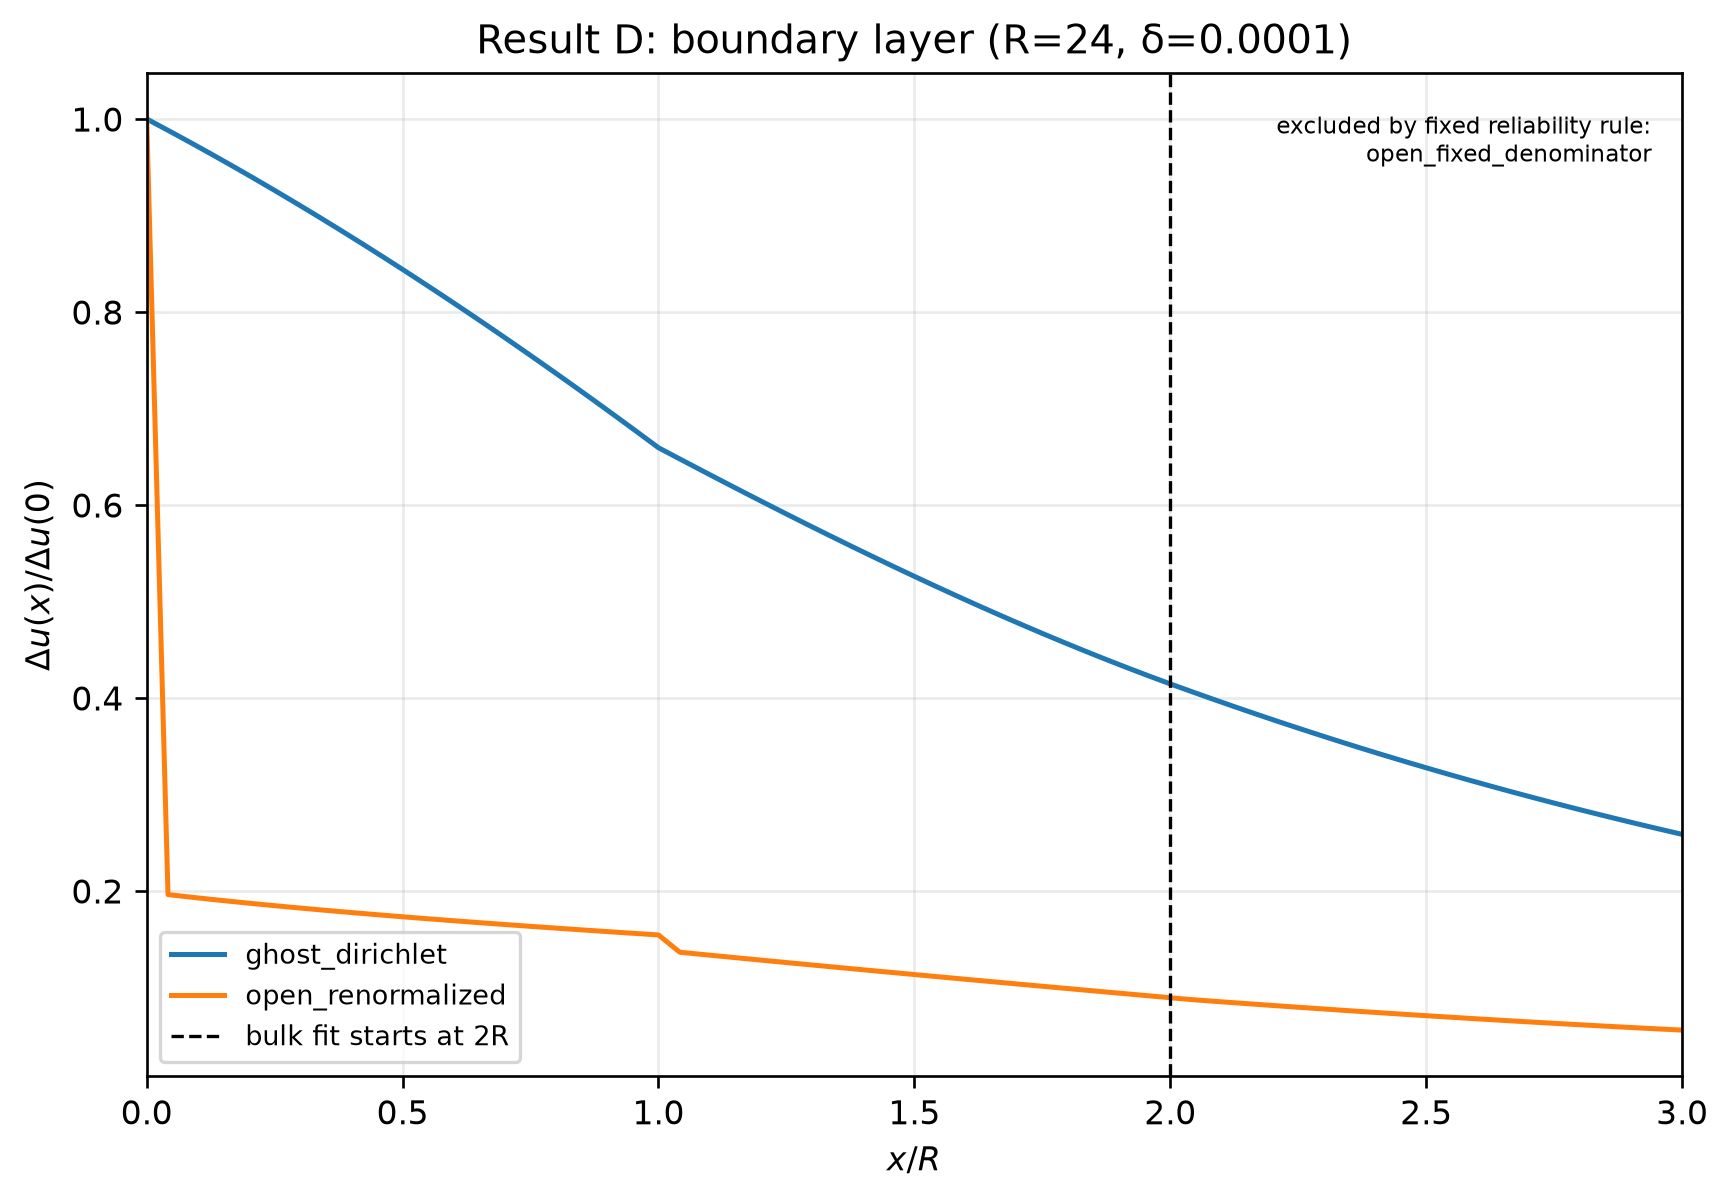
\includegraphics[width=0.82\linewidth]{figures/result3_boundary_layer.png}
\end{center}

左端からおよそ$2R$までは、欠けた近傍・固定値の扱いが局所平均を直接変える境界層である。
解析では
\begin{equation}
 x_{\min}=2R
 \label{eq:boundary-cutoff}
\end{equation}
を固定の保守的cutoffとして使う。$2R$は普遍的な境界厚さではない。

\begin{center}
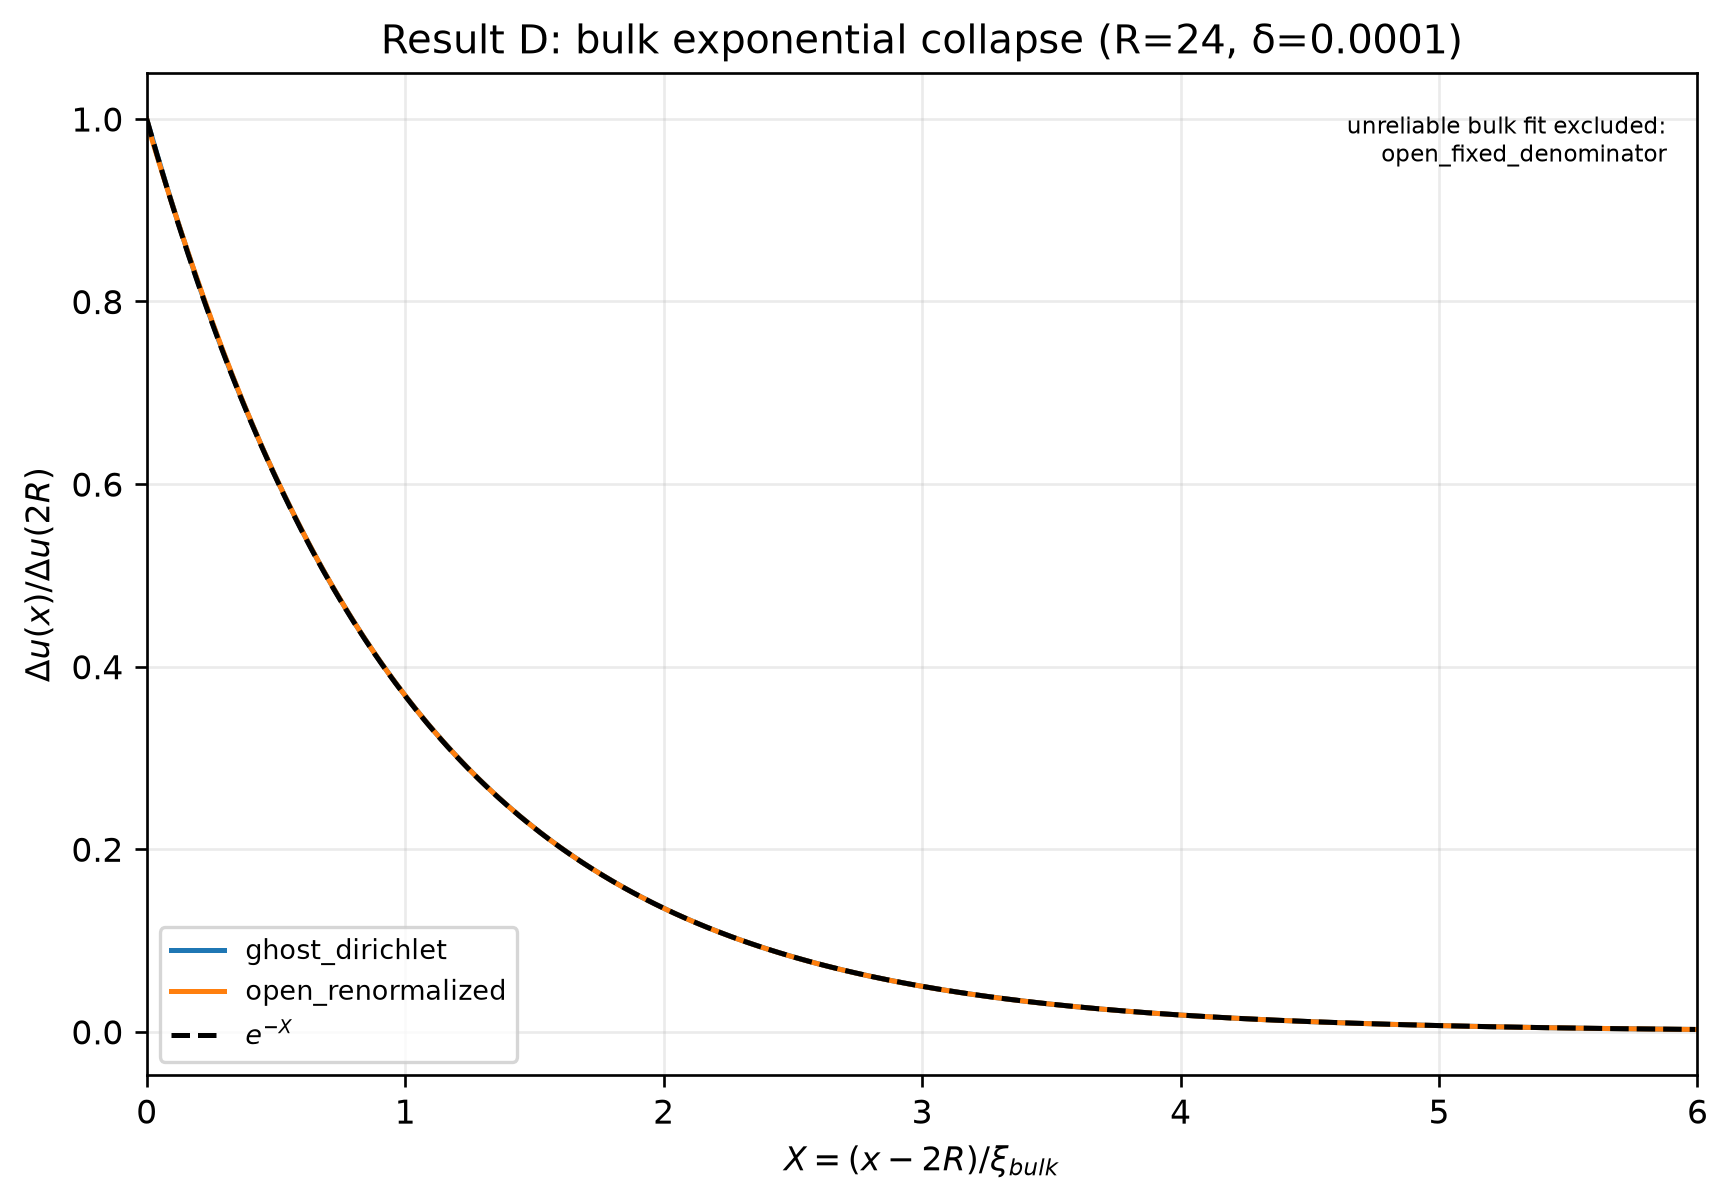
\includegraphics[width=0.82\linewidth]{figures/result3_bulk_collapse.png}
\end{center}

\section{境界条件ごとの注入振幅とbulk減衰}\label{sec:boundary-types}
\PosterMap{Result 3下段の「境界条件＝応答の大きさ」「内部領域＝到達距離」に対応。}

本計算で比較した境界実装は次の通りである。

\begin{description}[leftmargin=3.5em,style=nextline]
 \item[ghost Dirichlet]
 左端外側のghostサイトを指定値で埋め、分母を$2R$に保つ。
 \item[open renormalized]
 左端外側の欠けた近傍を除き、利用可能な近傍数で局所平均を規格化する。
 \item[open fixed denominator]
 欠けた近傍を除く一方で分母を$2R$に固定する診断条件。
 固定reliability基準を満たさず、ポスターのbulk collapseから除外した。
\end{description}

境界からbulkへ残る相対振幅を一例として
\begin{equation}
 T_{\bnd}\equiv\frac{\Delta u(2R)}{\Delta u(0)}
 \label{eq:T-bnd}
\end{equation}
と置ける。境界規則は主に$T_{\bnd}$、すなわちbulkへの注入振幅を変える。

bulk形状の比較では、境界条件ごとに独立fitした$\xi_{\bulk}$を使い、
\begin{equation}
 X=\frac{x-2R}{\xi_{\bulk}},\qquad
 Y=\frac{\Delta u(x)}{\Delta u(2R)}
 \label{eq:bulk-normalization}
\end{equation}
と規格化する。$x\ge2R$で
\begin{equation}
 Y\simeq\e^{-X}
 \label{eq:bulk-exp-collapse}
\end{equation}
へ重なることは、共通の指数関数形を支持する。

\Caution{
  式\eqref{eq:bulk-normalization}は各境界条件で得た$\xi_{\bulk}$を横軸へ使う。
  したがってcollapseだけから「すべての境界条件で$\xi$が完全に同じ」とは結論できない。
  Diehlの境界臨界現象\cite{diehl1997}は概念的背景であり、
  本非平衡離散写像が同じequilibrium boundary universality classに属するという主張でもない。
}

\section{Theoryと数値計算の対応表}\label{sec:correspondence}
\PosterMap{「数値検証」とResult 1--3を横断。}

\begin{longtable}{p{0.15\linewidth}p{0.22\linewidth}p{0.26\linewidth}p{0.18\linewidth}}
\toprule
項目 & 理論量 & 数値推定量・protocol & 注意 \\
\midrule
\endhead
一様固定点 & $F(u^*)=u^*$ & root solverで準安定枝を選択 & 近い不安定根を選ばない \\
一様倍率 & $\Lambda^*=F'(u^*)$ & $A_0(t+1)=\lambda A_0(t)$の原点通過fit & $\lambda(0)=\Lambda^*$ \\
時間率 & $\Gamma_0=-\ln\Lambda^*$ & $-\ln|\lambda_{\mathrm{fit}}(0)|$ & Result 2はfully numerical \\
時間スケール & $\tau_0=1/\Gamma_0$ & 数値$\Gamma_0$の逆数 & theory fallbackは不使用 \\
有限$q$倍率 & $\Lambda^*K_R(q)$ & $\pm\epsilon$応答の余弦振幅比 & closureとmicroを区別 \\
Result 1 & $\lambda(q)/\lambda(0)=K_R(q)$ & microの規格化ensemble response & 普遍的$q^2$証明ではない \\
格子長 & 式\eqref{eq:finite-R-characteristic}の$\xi_{\mathrm{lat}}$ & $\Gamma_{0,\mathrm{num}}$を代入して数値求根 & finite-$R$ bulk予測 \\
漸近理論長 & $\xi_{\Gamma}=\sqrt{\kappa_R/\Gamma_0}$ & theory referenceのみ & Result 2の横軸へ直接使用しない \\
境界長 & cosh/expの$\xi_{\bnd}$ & forced$-$baseline profileを独立fit & primaryはcosh、$x\ge2R$ \\
Result 2 & theory: $\tau_0=\xi_{\Gamma}^2/\kappa_R$ & test: $\tau_{0,\mathrm{num}}\simeq\xi_{\bnd}^2/\kappa_R$ & 同一closure内の別protocol \\
Result 3振幅 & 境界条件依存 & $T_{\bnd}=\Delta u(2R)/\Delta u(0)$ & injectionの違い \\
Result 3形状 & $\e^{-X}$ & 境界別$\xi_{\bulk}$で規格化 & $\xi$同一の証明ではない \\
\bottomrule
\end{longtable}

\section{主要な近似・成立条件一覧}\label{sec:assumptions}
\PosterMap{ポスター全体の質疑用。式を使ってよい範囲を一覧化。}

\begin{enumerate}
 \item \textbf{Gaussian結合和：}
 $J$がGaussianで独立、$S=\pm1$を条件とする限り有限$R$でも厳密。
 \item \textbf{Gaussian closure：}
 局所二値配置を局所平均$\bar u_i^{(R)}$で置き換え、
 quenched閾値と状態の動的相関、高次相関を明示追跡しない。
 \item \textbf{線形応答：}
 $\epsilon$が十分小さく、固定点のbasin内にある。対称差分の残差は$O(\epsilon^3)$。
 \item \textbf{Fourier分離：}
 bulkが並進対称で、周期境界を用いる。固定境界ではbulk近似として使う。
 \item \textbf{長波長展開：}
 $|q|Ra\ll1$、または実空間で$\xi\gg Ra$。
 有限$R$格子式\eqref{eq:finite-R-characteristic}自体はこの展開を使わない。
 \item \textbf{spinodal則：}
 Gaussian写像の非退化foldで$G_\Delta\neq0$、$G_{uu}\neq0$。
 \item \textbf{減衰率：}
 $\Gamma=-\ln|\lambda|$。$\lambda<0$では符号反転を包絡から分離する。
 \item \textbf{連続体境界式：}
 spinodal近傍かつbulkでゆっくり変化するprofile。有限系ではcoshを使う。
 \item \textbf{境界fit：}
 $x<2R$を除外するが、$2R$を普遍的境界厚さとは解釈しない。
 \item \textbf{有限$R$ microscopic：}
 operational pseudospinodalとmatched座標$s$を用いる。
 true spinodalや普遍指数を確立したとは述べない。
 \item \textbf{Result 2：}
 二つの独立モデルではなく、同じ局所平均意思の漸化式に対する
 時間・空間の別observable／別protocolの整合性検証。
 \item \textbf{Result 3：}
 規格化collapseは指数関数形を支持するが、境界別$\xi$の完全一致を示さない。
\end{enumerate}

\subsection*{Q\&A backup：数値robustness}
\addcontentsline{toc}{subsection}{Q\&A backup：数値robustness}

\textbf{境界forcing振幅。}
主解析窓$\delta_{\Gauss}\le3\times10^{-4}$で
$\epsilon_{\mathrm{fraction}}=0.025,0.10$を基準値0.05と比較すると、
$\xi_{\bnd}$の平均絶対相対差は$0.113\%$、最大$0.234\%$であった。

\begin{center}
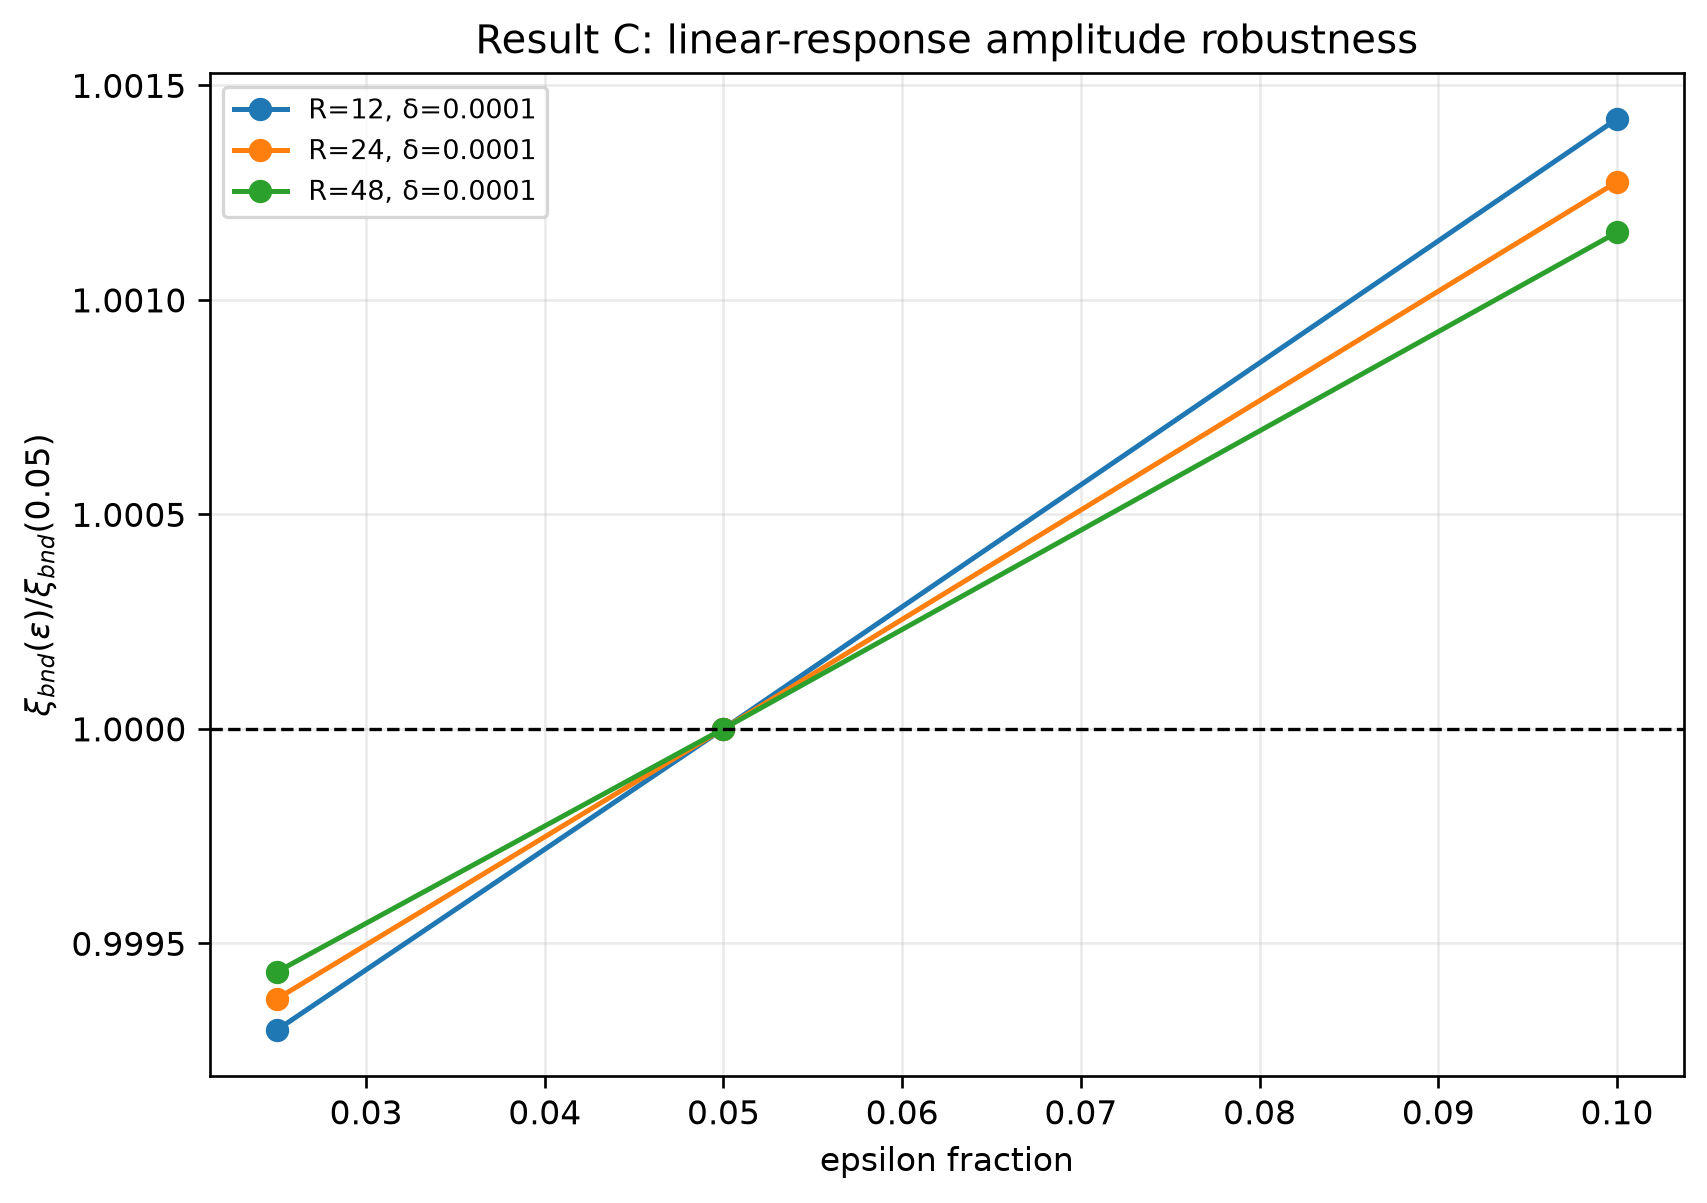
\includegraphics[width=0.82\linewidth]{figures/robustness_epsilon.png}
\end{center}

\textbf{fit開始位置。}
$x_{\min}=R,3R$をprimaryの$2R$と比較した同じ主解析窓では、
平均絶対相対差$0.160\%$、最大$0.822\%$であった。

\begin{center}
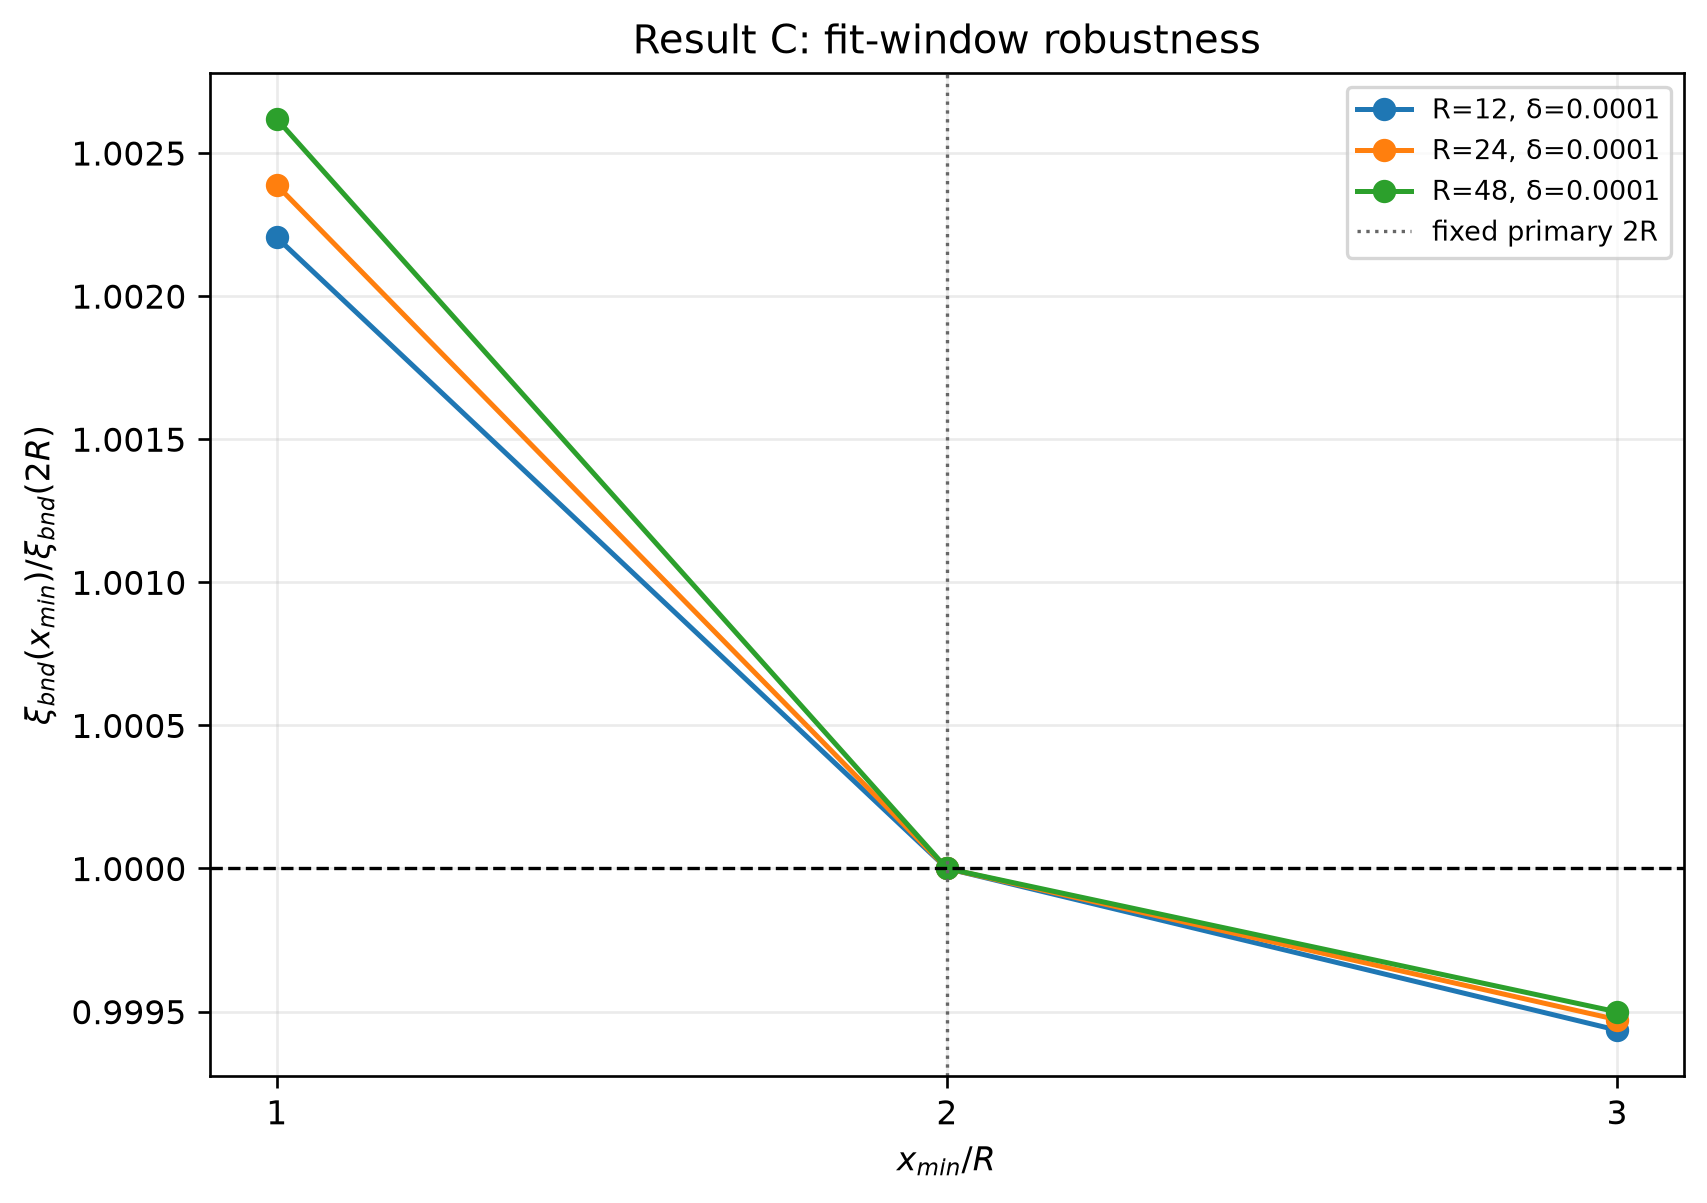
\includegraphics[width=0.82\linewidth]{figures/robustness_fitwindow.png}
\end{center}

\textbf{microscopic finite-size / seed control。}
次の2図はResult 2の決定論的closureではなく、microscopic matched responseの補助診断である。

\begin{center}
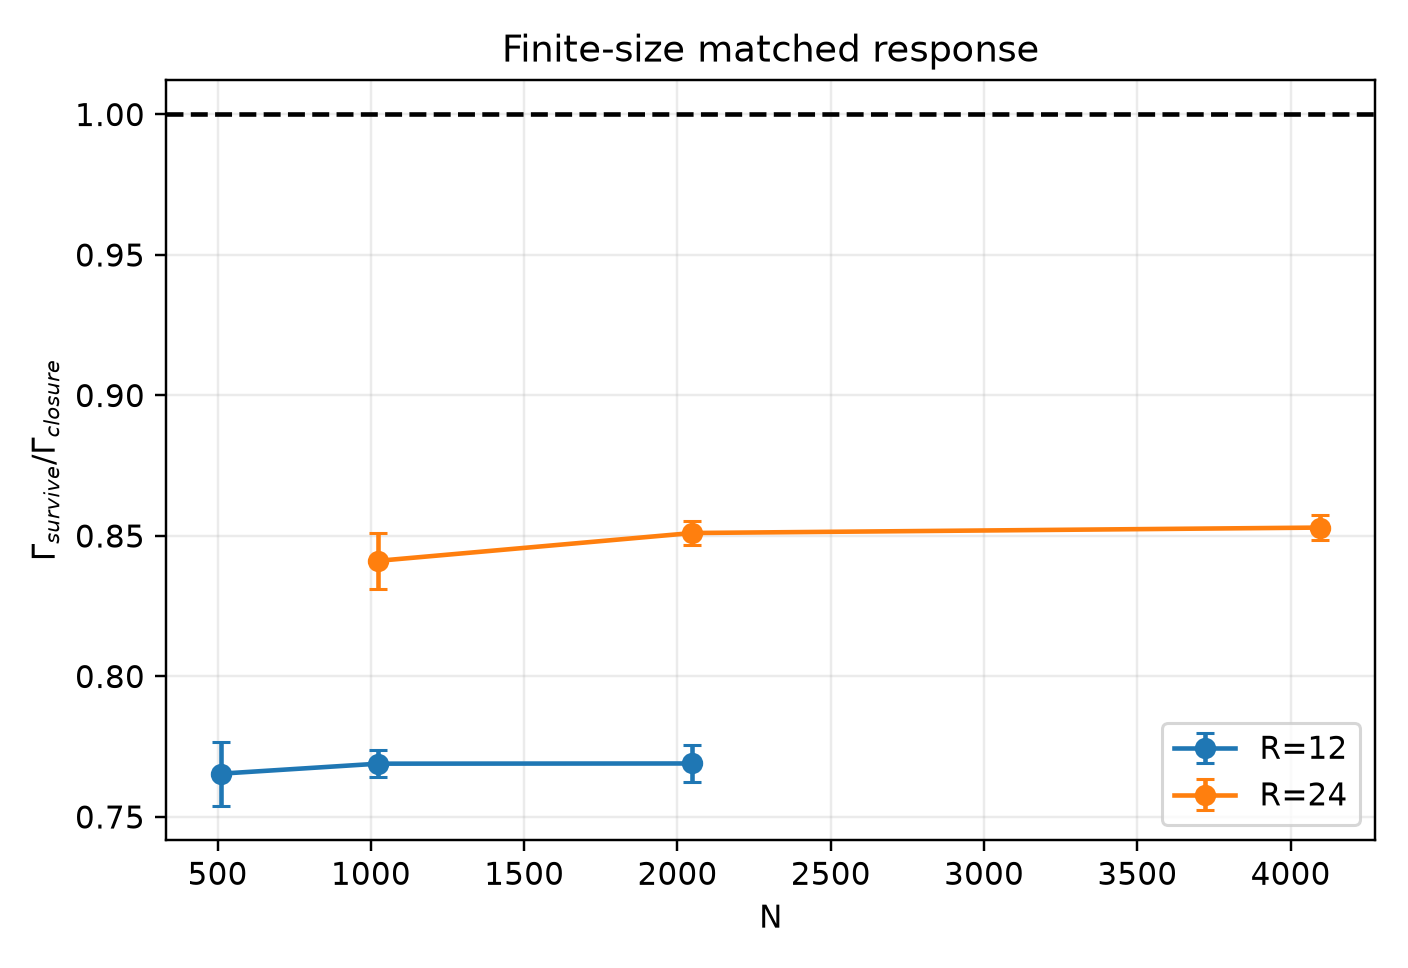
\includegraphics[width=0.78\linewidth]{figures/robustness_finite_size_gamma.png}

\vspace{0.5em}
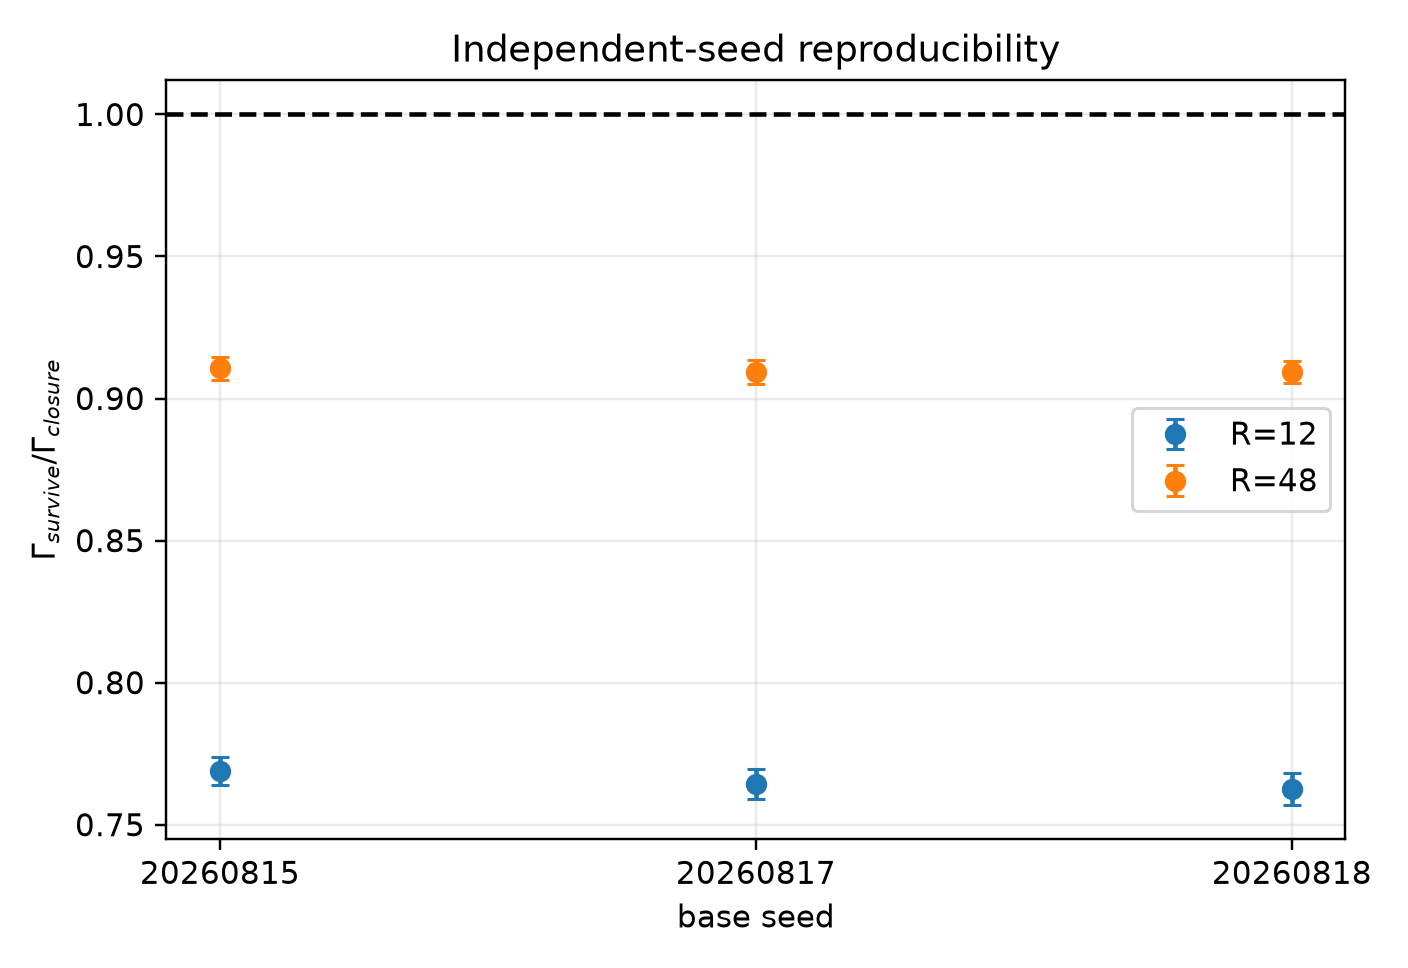
\includegraphics[width=0.78\linewidth]{figures/robustness_seed.png}
\end{center}

\textbf{observation timeとpseudospinodal。}
$\delta_{\mathrm{ps}}$が$T_{\mathrm{obs}}$依存であること自体が、
式\eqref{eq:pseudospinodal-criterion}が熱力学的臨界点でなくoperational criterionである証拠である。

\begin{center}
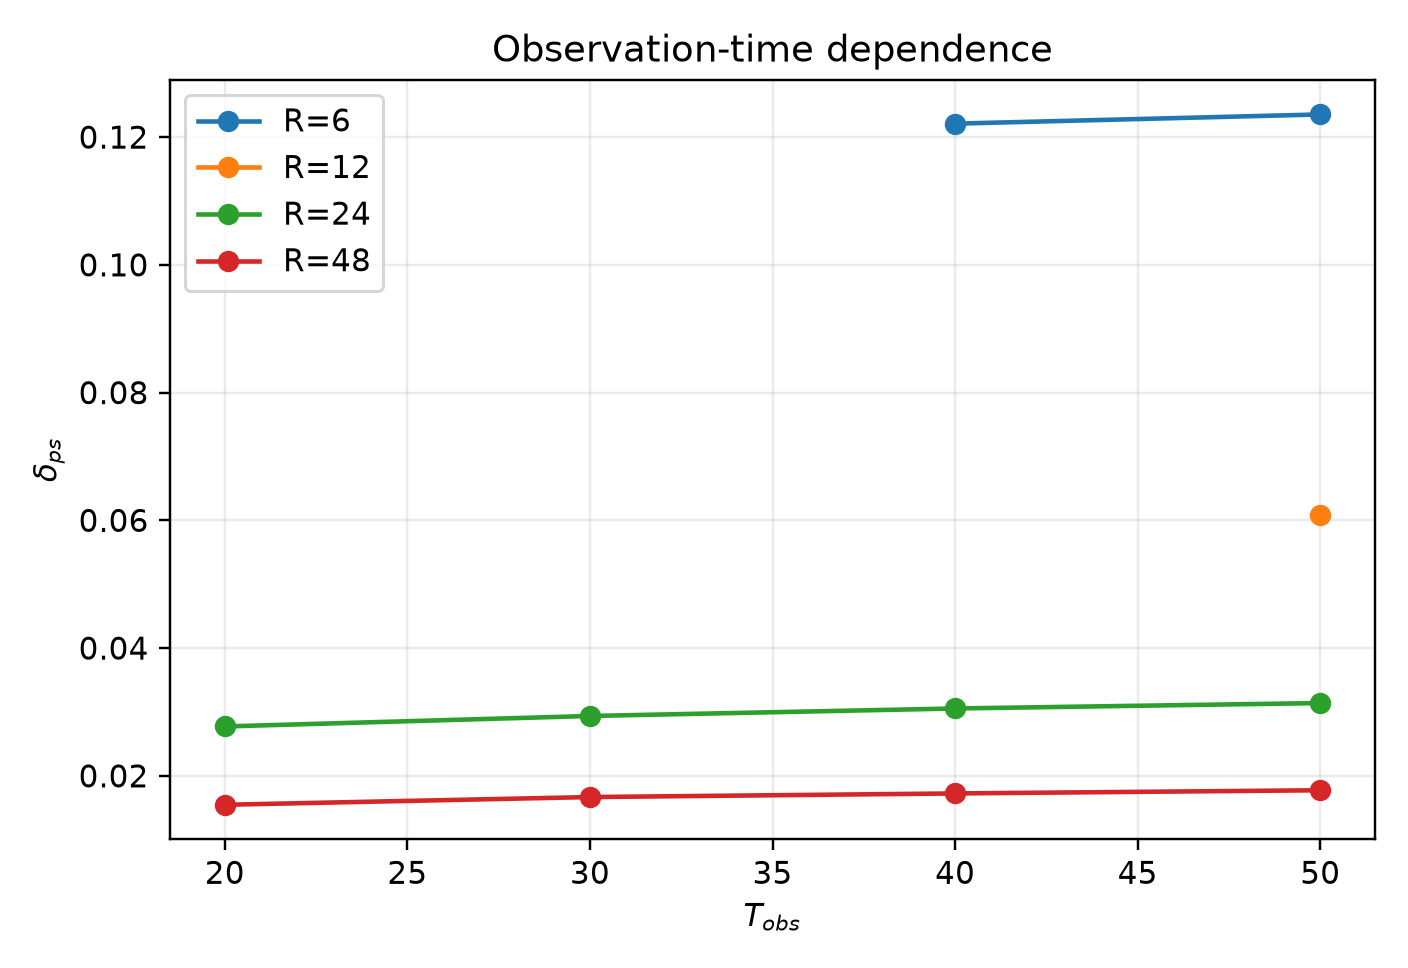
\includegraphics[width=0.78\linewidth]{figures/robustness_observation_time.png}
\end{center}

\clearpage
\section{想定質問から式を引くための索引}\label{sec:q-index}
\PosterMap{発表中の即時参照用。質問から節・式へ移動。}

\small
\begin{longtable}{p{0.41\linewidth}p{0.50\linewidth}}
\toprule
想定質問 & 見るべき節・式／短い答え \\
\midrule
\endhead
微視的モデルの更新式は？ & \hyperref[sec:microscopic]{第\ref*{sec:microscopic}節}、
式\eqref{eq:micro-field}, \eqref{eq:micro-update}。二値状態を局所場の符号で同期更新。 \\
$J$はquenched random bondか？ & \hyperref[sec:microscopic]{第\ref*{sec:microscopic}節}。
$J$は時刻ごとに更新するannealed乱数。quenchedなのは$\phi_i$。 \\
なぜ局所場はGaussianか？ & \hyperref[sec:gaussian-field]{第\ref*{sec:gaussian-field}節}、
式\eqref{eq:conditional-gaussian}。Gaussian $J$の線形和なので条件付きでは有限$R$でも厳密。 \\
どこが近似か？ & \hyperref[sec:closure]{第\ref*{sec:closure}節}と
\hyperref[sec:assumptions]{第\ref*{sec:assumptions}節}。局所配置と相関を平均意思だけで閉じる段階。 \\
$\sigma_{\mathrm{eff}}$は？ & 式\eqref{eq:sigma-eff}。
$J$和の分散$\sigma_J^2/(2R)$と閾値分散$\sigma_\phi^2$の和。 \\
局所平均意思の漸化式は？ & 式\eqref{eq:closure-map}。
正の局所場確率を$2P(+1)-1$へ変換。 \\
微視的モデルとclosureは同じか？ & \hyperref[sec:closure]{第\ref*{sec:closure}節}。
前者は$S_i=\pm1$を更新、後者は$u_i\in[-1,1]$を決定論的に更新。 \\
固定点の意味は？ & 式\eqref{eq:fixed-point}。
1ステップ後も変わらない一様な集団状態。 \\
spinodal条件は？ & 式\eqref{eq:spinodal-conditions}。
$G=0$と$G_u=0$、すなわち固定点と接線条件。 \\
なぜ$\Gamma_0\propto\delta^{1/2}$か？ &
\hyperref[sec:spinodal-scaling]{第\ref*{sec:spinodal-scaling}節}、
式\eqref{eq:spinodal-normal-form}--\eqref{eq:gamma-sqrt}。fold展開で$x\propto\sqrt\delta$。 \\
なぜ$\tau_0\propto\delta^{-1/2}$か？ & 式\eqref{eq:tau-sqrt}。
$\tau_0=1/\Gamma_0$。 \\
$\delta u_i$とは何か？ & \hyperref[sec:fourier]{第\ref*{sec:fourier}節}、式\eqref{eq:fourier-mode}。
理論では$u_i-u^*$。数値対称応答とは区別。 \\
なぜ$q=0$を使うか？ & \hyperref[sec:lambda-kernel]{第\ref*{sec:lambda-kernel}節}。
空間一様モードで$K_R(0)=1$、有限距離kernelによらず$\lambda(0)=\Lambda^*$だから。 \\
$q$が小さい／大きいとは？ & \hyperref[sec:fourier]{第\ref*{sec:fourier}節}。
小$q$は広域な偏り、大$q$は細かな局所差。 \\
$\lambda(q)=\Lambda^*K_R(q)$はどこから？ & 式\eqref{eq:spatial-linear}へ
Fourier modeを代入。導出は\hyperref[sec:lambda-kernel]{第\ref*{sec:lambda-kernel}節}。 \\
なぜ規格化するのか？ & 式\eqref{eq:normalized-spectrum}。
$\Lambda^*$を消し、$R$が決めるkernel形状だけを見るため。 \\
なぜ$\pm\epsilon$の差を取るのか？ & \hyperref[sec:symmetric]{第\ref*{sec:symmetric}節}、
式\eqref{eq:symmetric-difference}。背景と偶数次非線形を消す。 \\
同じ乱数を使う理由は？ & \hyperref[sec:symmetric]{第\ref*{sec:symmetric}節}。
正負差の分散を下げる。線形抽出自体は対称差分の役割。 \\
$\kappa_R$はfitしたのか？ & 式\eqref{eq:kappa-R}。
kernelの$\sum r^2$から解析的に決まる。 \\
なぜ$\Gamma(q)=\Gamma_0+\kappa_Rq^2$か？ &
\hyperref[sec:dispersion]{第\ref*{sec:dispersion}節}、式\eqref{eq:gamma-dispersion}。
$-\ln K_R(q)$の長波長展開。 \\
微視的$q^2$則を証明したか？ & \hyperref[sec:result1]{第\ref*{sec:result1}節}。
していない。Result 1の中心は規格化有限$q$ spectrumとkernelの整合。 \\
有限$R$ latticeでは$\xi$をどう決める？ &
\hyperref[sec:xi]{第\ref*{sec:xi}節}、式\eqref{eq:finite-R-characteristic}。
$1=\Lambda^*R^{-1}\sum_r\cosh(ra/\xi_{\mathrm{lat}})$の正根。 \\
$\xi=\sqrt{\kappa_R/\Gamma_0}$は有限$R$で厳密か？ &
厳密ではない。$\xi_{\Gamma}$は$\xi\gg Ra$かつ$\Gamma_0\ll1$の漸近式。
順序は式\eqref{eq:finite-R-characteristic}--\eqref{eq:xi-Gamma}。 \\
$\xi_{\mathrm{lat}}$と$\xi_{\bnd}$は一致するか？ &
\hyperref[sec:result2]{第\ref*{sec:result2}節}。全20条件で平均差$0.147\%$、最大差$0.226\%$。 \\
full finite-$R$ kernelとcontinuum $q^2$近似の差は？ &
式\eqref{eq:finite-R-characteristic}と\eqref{eq:xi-Gamma}。20条件で
$|\xi_{\Gamma}/\xi_{\mathrm{lat}}-1|$は平均$0.372\%$、最大$0.903\%$。 \\
なぜ$\xi\propto\delta^{-1/4}$か？ & \hyperref[sec:xi-scaling]{第\ref*{sec:xi-scaling}節}、
式\eqref{eq:xi-quarter}。$\Gamma_0\propto\delta^{1/2}$の平方根逆数。 \\
なぜ$z=2$か？ & \hyperref[sec:z2]{第\ref*{sec:z2}節}、式\eqref{eq:tau-xi}, \eqref{eq:z-two}。
固定$R$で理論長$\xi_{\Gamma}$に対し$\tau_0=\xi_{\Gamma}^2/\kappa_R$。 \\
$\tau=\xi^2/\kappa_R$は定義か数値検証か？ &
理論では$\xi_{\Gamma}$の定義から等号。独立fitした$\xi_{\bnd}$には
式\eqref{eq:tau-xi-numeric-test}の近似等号を検証する。 \\
Model Aを証明したか？ & \hyperref[sec:z2]{第\ref*{sec:z2}節}。
していない。非保存Gaussian長波長予測との整合を示す。 \\
Result 2は二つのモデルの独立検証か？ & \hyperref[sec:result2]{第\ref*{sec:result2}節}。
同じclosure内で、周期$q=0$時間緩和と固定境界空間応答を別々に測る整合性検証。 \\
$\xi$は理論式から計算したか？ & 式\eqref{eq:tau-numeric}周辺。
Result 2・3の$\xi_{\bnd}$は境界profileから独立fit。 \\
なぜ$R$をまたぐと$\xi/\sqrt{\kappa_R}$か？ &
\hyperref[sec:result2]{第\ref*{sec:result2}節}、式\eqref{eq:xi-scaled}。
kernel由来の既知の$R$依存prefactorを除くため。 \\
$R$ sweepで何を固定している？ & \hyperref[sec:result2]{第\ref*{sec:result2}節}。
$B=2,\sigma_J=1,\sigma_\phi=0.06,\bar\phi=0,a=1$、枝とforcing比を固定。 \\
$\mu$は$R$によって変えるか？ & 式\eqref{eq:mu-fixed-B}。$B$固定のため
$\mu(R)\propto\sigma_{\mathrm{eff}}(R)$として変える。 \\
同じabsolute $\delta$は同じ臨界距離か？ & 式\eqref{eq:reduced-delta}。
$\widetilde\delta=\delta_{\Gauss}/\sigma_{\mathrm{eff}}(R)$は$R$依存なので完全には同じでない。 \\
$z_{\mathrm{eff}}=1.984$をどう言う？ & \hyperref[sec:result2]{第\ref*{sec:result2}節}。
有限距離指数は2より少し小さく、spinodalに近い窓で2へ接近。統計的証明とは言わない。 \\
$R=6$でもなぜ$z\simeq2$が見える？ & \hyperref[sec:R6]{第\ref*{sec:R6}節}、
式\eqref{eq:scale-separation}。重要なのは$R\to\infty$より$\xi\gg Ra$；格子式でも直接確認。 \\
有限系でなぜcoshか？ & \hyperref[sec:cosh]{第\ref*{sec:cosh}節}、
式\eqref{eq:finite-L-cosh}。右端反射条件を指数関数の一般解へ課す。 \\
Result 3の$\Delta u$は？ & 式\eqref{eq:boundary-response}。
同じ境界規則でforcedからbaselineを引いた定常応答。 \\
boundary forcingはいくらか？ & 式\eqref{eq:boundary-forcing}。
spinodal方向へ$|u_{\mathrm{sp}}-u^*|$の5\%を左端に与える。 \\
$\epsilon$を変えても結果は同じか？ & \hyperref[sec:assumptions]{第\ref*{sec:assumptions}節}のbackup。
主窓で$\xi_{\bnd}$の平均差$0.113\%$、最大$0.234\%$。 \\
$x_{\min}$を$2R$から変えても同じか？ & 同backup。
$R,3R$との比較で平均差$0.160\%$、最大$0.822\%$。 \\
なぜ$x<2R$を除く？ & 式\eqref{eq:boundary-cutoff}。
境界規則が局所平均へ直接入る領域を保守的に除く。普遍厚さではない。 \\
境界条件は何を変える？ & 式\eqref{eq:T-bnd}。
主にbulkへ入る注入振幅を変える。 \\
境界条件で$\xi$は同じか？ & \hyperref[sec:boundary-types]{第\ref*{sec:boundary-types}節}。
規格化collapseだけでは完全同一と言えない。境界ごとに$\xi$をfitしている。 \\
finite-$R$ microscopicのspinodalは？ & \hyperref[subsec:two-distances]{第\ref*{subsec:two-distances}節}。
真のspinodalとは断定せずoperational pseudospinodalと呼ぶ。 \\
pseudospinodalを具体的にどう決めた？ & 式\eqref{eq:pseudospinodal-criterion}。
$T_{\mathrm{obs}}=50$で累積escape確率が0.10を横切る補間位置。 \\
\bottomrule
\end{longtable}
\normalsize

\clearpage
\section*{資料間の定義差と本資料での判断}
\addcontentsline{toc}{section}{資料間の定義差と本資料での判断}

\begin{itemize}
 \item \textbf{最新版：}ユーザー指定の
 \texttt{2026年秋学会ポスター\_v2.pptx}を優先した。
 \item \textbf{Gaussian化：}予稿・旧スライドの「CLT」表現を、
 Gaussian $J$の条件付き和は厳密、平均意思だけで閉じる段階は近似、と分解した。
 \item \textbf{記号：}予稿は一様固定点を$m^*$、ポスターと現在の局所場説明は$u_i$を用いる。
 本資料は局所平均を$u_i$、一様固定点を$u^*$へ統一した。
 \item \textbf{距離：}Gaussian spinodal距離$\delta_{\Gauss}$と、microscopic matched座標$s$を分離した。
 \item \textbf{特徴長：}finite-$R$格子根$\xi_{\mathrm{lat}}$、長波長漸近長$\xi_{\Gamma}$、
 境界profileの独立fit長$\xi_{\bnd}$を分離した。
 \item \textbf{Result 2：}ポスターv2と現コードに合わせ、同一closure内の別protocol・別observableとした。
 \item \textbf{Result 3：}境界別の独立fit長で規格化するため、collapseを$\xi$同一の証明と解釈しない。
\end{itemize}

\clearpage
\section*{参考文献と研究資料}
\addcontentsline{toc}{section}{参考文献と研究資料}
\nocite{poster2026,proceedings2026,repository2026}
\printbibliography[heading=none]

\end{document}
